\documentclass[10pt, landscape, a4paper]{article}
\usepackage{geometry}[landscape]
\usepackage{multicol}
\usepackage{graphicx}
\usepackage{amsmath} 
\usepackage{amssymb}

\usepackage[dvipsnames]{xcolor}

% Set page margins
\geometry{top=.8cm, left=.8cm, right=.8cm, bottom=.8cm}

% Set paragraph indentation
\setlength{\parindent}{0pt}

% Set path for assets
\graphicspath{{assets/}}

\setlength{\columnsep}{20pt}
\raggedcolumns

% _____ CUSTOM COMMANDS __________________________________________
\newcommand{\E}[0]{\mathbb{E}}
\newcommand{\R}[0]{\mathbb{R}}

\newcommand{\sgn}[0]{\text{sgn}}

\newcommand{\argmin}[1]{\underset{#1}{\text{argmin}}}
\newcommand{\argmax}[1]{\underset{#1}{\text{argmax}}}

\begin{document}
\begin{multicols*}{3}

% _____ CONTENT __________________________________________________

% main heading
\begin{center}
	\Large{\textbf{Introduction to Machine Learning}} \\
    \small{by dcamenisch}
\end{center}

\section{Introduction}

asdfhkajdsfhasöj

\section{Regression}

In this first part we are gonna focus on fitting lines to datapoints. For this we will introduce the \textbf{machine learning pipeline}. It consists of three parts and has the goal to find the optimal model $\hat{f}$ for given data $D$, that we can use to predict new data.

\smallskip

\includegraphics[width=\columnwidth]{ml-pipeline.png}

The three parts of the ML Pipeline are the function class $\mathbf{F}$, the loss function $\ell$ and the optimization method. \medskip

In the coming sections $f^*$ will be the ground truth function and $\hat f$ will be used for our (learned) prediction model.

\subsection{Linear Regression}

Given the data $(x_i, y_i)$ we use models of the form $f(x) = w^\top x + b$ to fit the data. To find the optimal values for $w$ and $b$ we try to reduce the \textbf{squared loss}:
$$\ell(y, f(x)) := \frac{1}{n}\sum (y_i - f(x_i))^2 = \frac{1}{n}||y - X w||_2^2$$

In the matrix notation $b$ is part of $w$. The closed form solution for linear regression is given by the normal equation $Ax - b \Rightarrow x = (A^\top A)^{-1} A^\top y$:
$$\hat{w} = (X^\top X)^{-1}X^\top y$$

We can also get the closed form solution by using the fact that the squared loss is a convex function and $\hat{w}$ is the global minima of this function. Therefore we can calculate the gradient $\nabla \ell(y, f(x))$ and solve for $0$ to find $\hat{w}$. Later, we will see a more efficient way of finding $\hat{w}$. \medskip

\subsubsection{Different Loss Functions}

The square loss penalizes over- and underestimation the same. Further it puts a large penalty on outliers (grows quadratically). While this is often good, we might want a different loss function, some possibilities are:

\begin{itemize}
	\item Huber loss - ignores outliers ($a = y - f(x)$
		$$\ell_\delta(y, f(x)) := \begin{cases}
			\frac{1}{2} a^2 & \text{for } |a| \leq \delta \\
			\delta \cdot (|a| - \frac{1}{2} \cdot \delta) & \text{otherwise}
		\end{cases}$$
	\item Asymmetric losses - weigh over- and underestimation differently
\end{itemize}

\subsection{Nonlinear Functions}

Linear functions helped us to keep the calculations "simple" and find good solutions. But often there are problems that are more complex and would require nonlinear functions. The avoid using nonlinear functions we introduce feature mapping. 

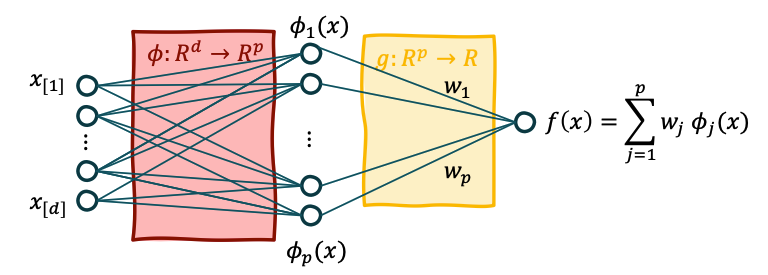
\includegraphics[width=\columnwidth]{feature-mapping.png}

From our input vector $x$ we extract a \textbf{feature vector} $\phi(x)$ by using a fixed mapping $\phi$ that can consist of any nonlinear function. On this feature vector we can use the already known methods for linear functions to find a solution.

\subsection{Regularization}

We will later see that too complex models are not always good, as they use too many features. If we want to reduce the number of features, we can encourage sparsity by introducing a penalty term. We commonly use:
\begin{itemize}
	\item \textbf{Lasso Regression}: $\argmin{w \in \R^d} ||y - \Phi w||^2 + \lambda ||w||_1$
	\item \textbf{Ridge Regression}: $\argmin{w \in \R^d} ||y - \Phi w||^2 + \lambda ||w||_2$
\end{itemize}

Lasso regression sets a lot of weights to zero, while ridge regression just puts the focus on lower weights.
\section{Optimization}

If the closed form is not available or desirable, as calculating it is expensive, we use the \textbf{gradient descent} algorithm. It works by initializing $w^0$ and iteratively moving it towards the optimal solution. We choose the direction by calculating $\nabla \ell(w)$ and then multiply it by the stepsize / learning rate $\eta$:
$$w^{t+1} = w^t - \eta_t \cdot \nabla \ell(w^t)$$

Convergence is only guaranteed for the convex case, else we might get stuck at any stationary point. 

\begin{center}
	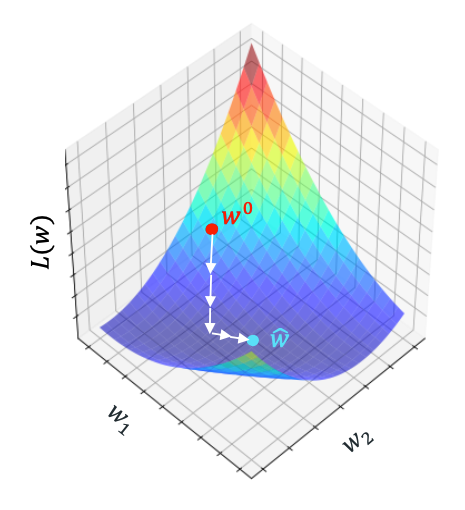
\includegraphics[width=0.6\columnwidth]{gradient-descent.png}
\end{center}

As the slope gets smaller, we want to decrease $\eta$, so that we do not overshoot. For the linear regression case we have:
$$||w^t - w^*||_2 \leq \rho^t ||w^0 - w^*||_2, \quad \rho = ||I - \eta X^\top X||_{op}$$

Where $\rho$ is the convergence speed for constant stepsize $\eta$. This leads to an optimal fixed stepsize of:
$$\eta = \frac{2}{\lambda_{\text{min}} + \lambda_{\text{max}}}$$

We stop when new iterations do not cause any change anymore (below a certain threshold).

To make gradient descent more stable / robust against ill-conditioned landscapes we might add momentum:
$$w^{t+1} = w^t + \gamma \Delta w^{t-1} - \eta_t \nabla \ell(w^t)$$

\subsection{Stochastic Gradient Descent}

When we have a lot of data, it is costly to compute the gradient, so we only use a minibatch $S$ of the dataset $D$ (randomly sampled without replacement). Now the update step looks like this:
$$w^{t+1} = w^t - \eta_t \cdot \nabla \ell_S(w^t)$$

Where the loss is only calculated over the minibatch $S$. This method also gives us a chance to escape saddle points.
\section{Model Error}

We generally want to minimize the estimation error $\ell(\hat{f}(x), f^*(x))$, since we do not know $f^*$ we can not actually compute this value. Instead, we usually observe $y_i = f^*(x_i) + \epsilon_i$. For each observed sample we can compute the \textbf{prediction error} $\ell(\hat{f}(x), y)$, in fact we are often interested in the average prediction error or \textbf{generalization error}:
$$R(\hat{f}) := \E_{x,y}[\ell(\hat{f}(x), y)] = \E_x[\ell(\hat{f}(x), f^*(x))] + \epsilon$$

The generalization error computed over all possible $(x,y)$ pairs weighted by how likely each is. 

The training loss is often to optimistic to approximate the generalization error. To get a better approximation we split our data into training and test set. 

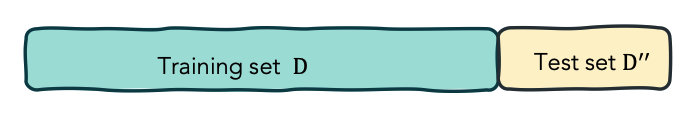
\includegraphics[width=\columnwidth]{train-test-split.png}

By only using the training set to fit our model, we have the test data to get a better estimate of the generalization error.

\subsection{Cross-Validation}

When choosing between different models, we might choose the model with the lowest test set error, this may introduce a systematic bias. To prevent this from happening we can split the training set again, creating a validation set. Now the idea is to choose the model with the best validation error and use the test set only to get the estimate for the generalization error.

Setting aside so much data can be wasteful. So we introduce \textbf{$k$-fold cross-validation}

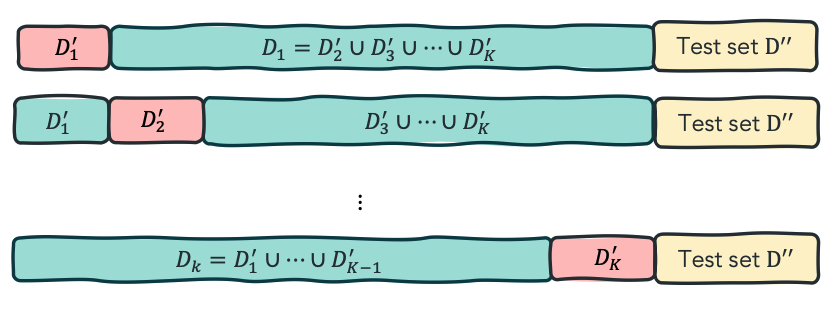
\includegraphics[width=\columnwidth]{cross-validation.png}

We proceed as follows:
\begin{enumerate}
	\item For all folds $k = 1,..., K$: 
		\begin{enumerate}
			\item Train $\hat{f}_k$ on $D' - D'_k$
			\item Compute val. error $R_k = \frac{1}{|D'_k|} \sum_{x,y} \ell(\hat{f}_k(x), y)$
		\end{enumerate}
	\item Compute cross-validation error $CV = \frac{1}{K} \sum_{i=1}^K R_i$
	\item Pick model with lowest cross-validation error $CV$
	\item Evaluate the model using the test set $D''$
\end{enumerate}

For $K$ very large, we can get the best approximation, if $K = |D'|$ we call it leave-one-out cross-validation (LOOCV).

\subsection{Model Complexity}

Model complexity is closely related to training and generalization error.

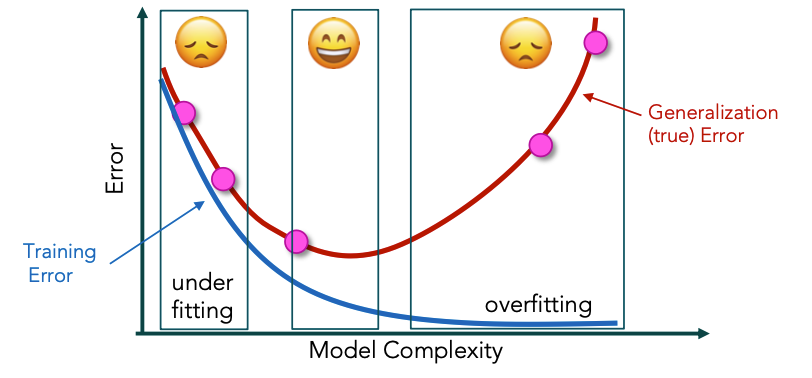
\includegraphics[width=\columnwidth]{overfitting.png}

\subsection{Bias and Variance}

For different datasets $D_1,...,D_K$ we define:
\begin{itemize}
	\item \textbf{Bias} - distance of the average model $\bar{f} = \frac{1}{K} \sum_{i=1}^K \hat{f}_i$ to the ground truth $\E_x[\ell(\bar{f}(x), f^*(x))]$
	\item \textbf{Variance} - average distance of the models to the average model $\E_x[\frac{1}{K} \sum_{i=1}^K \ell(\hat{f}_i(x), \bar{f}(x))]$
\end{itemize}

\begin{center}
	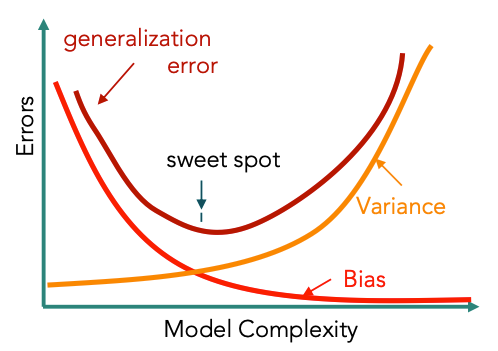
\includegraphics[width=0.8\columnwidth]{bias-variance-tradeoff.png}
\end{center}
\section{Classification}

Instead of predicting $y \in \R$, we limit $y$ to be in a finite, discrete set $Y$ (e.g. $\{-1, +1\}$). When looking at binary classification we often use the labels $-1, +1$ and let the predicted value be equal to $\hat{y} = \sgn\hat{f}(x)$. Similar to regression we care about the generalization error:
$$R(\hat{f}) = \mathbb{P}_{x,y} [y \neq \sgn \hat{f}(x)] = \E_{x,y}[\ell_{0-1}(\hat{f}(x), y)]$$

Where we call $\ell_{0-1}(\hat{f}(x), y) = \mathbb{I}_{y \neq \sgn \hat{f}(x)}$ the \textbf{zero-one loss}. Since this loss is neither convex nor continuous, we can not efficiently minimize the training error with it. Therefore we introduce different type of loss functions:
\begin{itemize}
	\item \textbf{Exponential loss}: $\ell_\text{exp}(\hat{f}(x), y) = e^{y \hat{f}(x)}$
	\item \textbf{Logistic loss}: $\ell_\text{log}(\hat{f}(x), y) = \log(1 + e^{y \hat{f}(x)})$
	\item \textbf{Hinge loss}: $\ell_\text{hinge}(\hat{f}(x), y) = \max(0, 1-y \hat{f}(x))$
	\item \textbf{Linear loss}: $\ell_\text{lin}(\hat{f}(x), y) = y \hat{f}(x)$
\end{itemize}

We will mainly focus on the logistic loss (also called \textbf{logistic regression}), as in practice it is the most used. We can derive that the logistic loss is the negative conditional $\log$ likelihood $\mathbb{P}[y = +1 | x]$ or $\mathbb{P}[y = -1 | x]$ that is parameterized by $\hat{f}(x)$ via the \textbf{softmax transformation}. We define (similar for $y = -1$): $$\mathbb{P}[y = +1 | x] = \frac{1}{1 + e^{- \hat{f}(x)}}$$

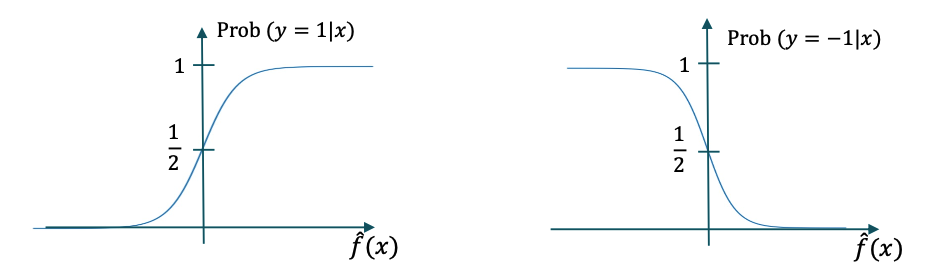
\includegraphics[width=\columnwidth]{conditional-probability.png}

Using this we can define the probability vector:
$$\hat{p}(x) = (\mathbb{P}[y = -1 | x], \; \mathbb{P}[y = +1 | x])$$

If we want to extend the log loss to multiple classes, we define a vector $\tilde{f}(x) = (\hat{f}_1(x), ..., \hat{f}_K(x))$ and transform it using softmax:
$$\hat{p}_k = \frac{e^{\hat{f}_k(x)}}{\sum_{i=1}^K e^{\hat{f}_j(x)}}$$

For the multiclass case we choose the classifier error to be the maximal entry of $\hat{p}$ if $y \neq \hat{y}$.

\subsection{Linear Classifiers}

Linear classifiers use functions form the class $F = \{ f \; | \; f(x) = w^\top x, \; w \in \R^d\}$. We already know that this class of functions makes training and prediction simple. The decision boundary of the function is given by $\{ x \; | \; f(x) = 0\}$.

\begin{center}
	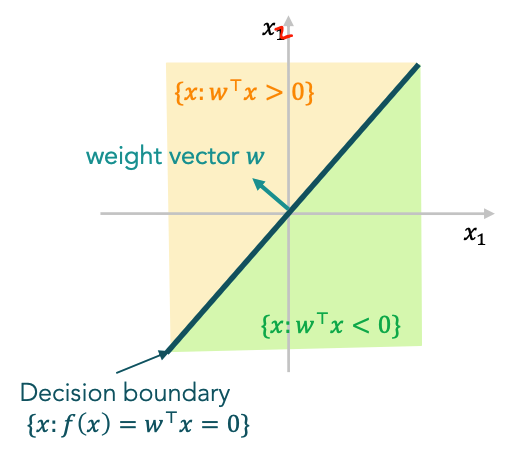
\includegraphics[width=0.64\columnwidth]{linear-classifiers.png}
\end{center}

To train our classifier we can use gradient descent. The gradient of the logistic loss is given by:
$$\nabla \ell(\hat{f}(x), y) = \frac{y_i x_i}{1 + e^{y_i \hat{f}(x)}}$$
 
 For linearly separable data, gradient descent on the logistic loss converges to the direction $w_\text{MM}$ that maximizes the minimum $\ell_2$-distance between the decision boundary and $y_i$. We call this the \textbf{maximum-margin} solution.
 
 In particular we can write:
 $$w_\text{MM} = \argmax{||w||_2 = 1} \min_i y_i w^\top x_i = \argmax{||w||_2 = 1} \; \text{margin} (w)$$
 
 Instead of just linear functions, we can again use feature mapping to receive nonlinear classifiers.
 
 \subsection{Support Vector Machines}
 
 For general $w$ that correctly separates the data, $\frac{\text{margin}(w)}{||w||_2}$ is the min. distance of any point to the decision boundary. If we use general $w$ the solution is not unique anymore. But we can rescale any unit norm $w$ by $\alpha = \frac{1}{\text{margin}(w)}$ such that $\alpha w = \tilde{w}$. So instead of searching within unit norm $w$ to find $w_\text{MM}$ with maximum margin, we can search within all $\tilde{w}$ with margin$(\tilde{w}) = 1$ to find the one that maximizes:
 $$\frac{\text{margin}(\tilde{w})}{||\tilde{w}||_2} = \frac{1}{||\tilde{w}||_2}$$ 
 
 This is how support vector machines work. More formal:
 $$\hat{w} = \min_w ||w||_2 \quad \text{s.t. } y_i w^\top x_i \geq 1 \text{ for all } i=1,...,n$$
 
 If the data is not linearly separable, we might want to use a \textbf{soft-margin SVM}. Since not all constraints can hold, we want to allow some "slack" in the constraints:
 
  $$\hat{w} = \min_{w, \xi} \frac{1}{2} ||w||_2^2 + \lambda \sum_{i=1}^n \max (0, 1 - y_i w^\top x_i)$$
  
  The later part penalizes any margin violations. To find the optimal $\lambda$ one might use cross-validation.
  
\section{Hypothesis Testing}

We focused a lot to derive good surrogate losses for the 0-1 loss. But is this error really a good metric? Hypothesis testing is a way to express asymmetry in classification tasks. For this we introduce the confusion matrix:

\begin{center}
	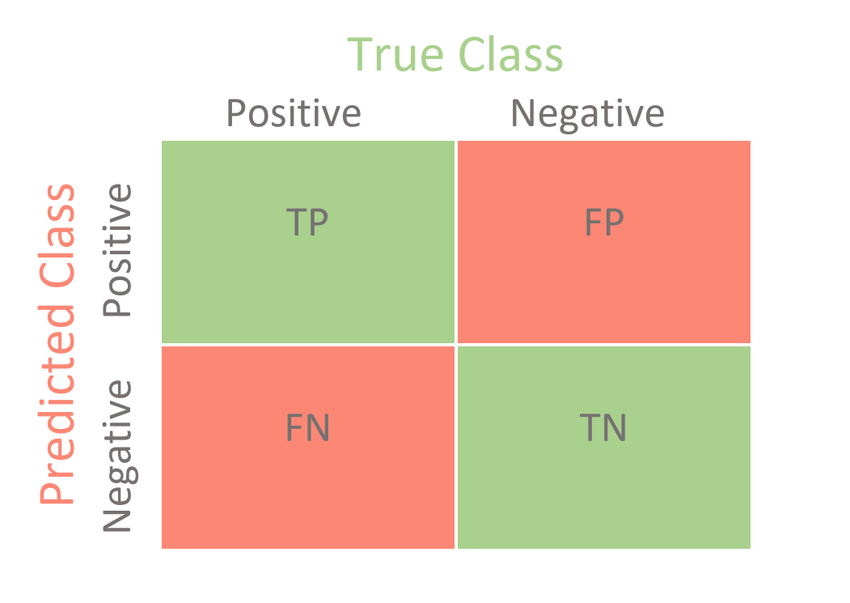
\includegraphics[width=0.85\columnwidth]{confusion-matrix.png}
\end{center}

Further we define:
$$\text{error}_1 / \text{FPR} = \frac{FP}{TN + FP}, \quad \text{error}_2 / \text{FNR} = \frac{FN}{TP + FN}$$

We want to find a test that minimizes the FPR, while controlling the FNR. This can be viewed as defining a null hypothesis $H_0(x)$ and then deciding to accept or reject it ($H_0$ is always the positive class). When choosing $H_0$ we want it to represent the more crucial class one to get right, e.g. it is more important to truly classify a person as sick than to classify them as healthy. To decide it we accept or reject $H_0$ we fix $\tau$, where we accept $H_0(x) (\hat{y} = -1)$ if $\hat{p}(x) < \tau$ and the opposite way around.

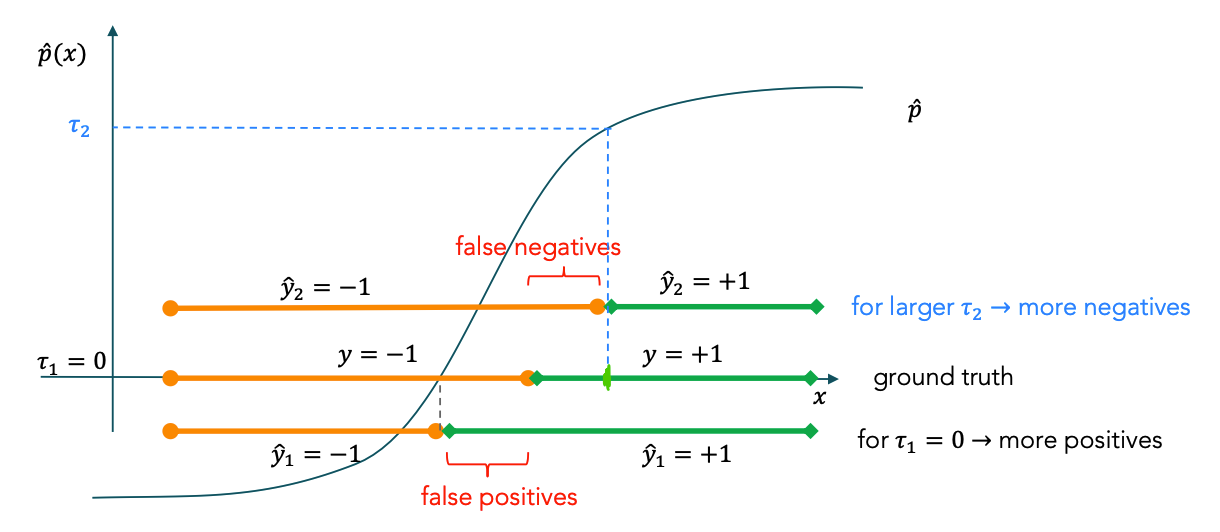
\includegraphics[width=\columnwidth]{fp-fn-tradeoff.png}

\subsection{AUROC}

We want to have a large recall $\frac{TP}{\#[y = +1]}$ but also a small FPR. Based on these metrics we can draw the ROC curve by varying $\tau$.

\begin{center}
	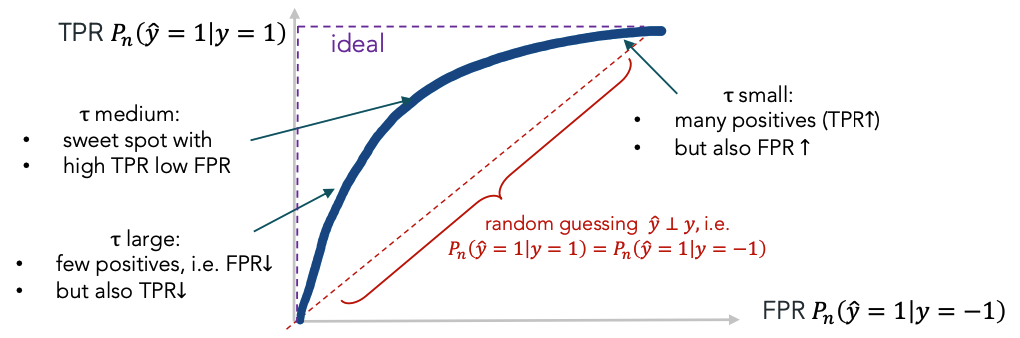
\includegraphics[width=0.87\columnwidth]{roc.png}
\end{center}

We can either choose our model by caring about a specific point, e.g. TPR $@$ FPR = 5\%, or we choose whichever courve gets closer to the ideal curve, that is maximizing the area under the curve.
\section{Kernels}

We have previously seen how we can get nonlinear functions via feature maps $\phi$. But there are limits to these feature maps, they can introduce a lot of computational complexity (feature explosion) and there are also infinite feature maps we can not get this way. If we want to avoid these limitations we use the \textbf{kernel trick}. It consists of two steps:

\begin{enumerate}
	\item We know that the solution $\hat{w}$ is in the column space of $\Phi^\top$. Therefore among the global minimizers one has the form $\hat{w} = \Phi^\top \hat{\alpha}$ with $\hat{\alpha} \in \R^n$ so that:
		$$\hat{f}(x) = \hat{w}^\top \phi(x) = \hat{\alpha}^\top \Phi \phi(x) = \sum_{i=1}^n \hat{\alpha}_i \cdot \phi(x_i)^\top \phi(x)$$
		Notice that $\hat{\alpha}$ only depends on $x_i$ via inner products $\phi(x_i)^\top \phi(x_j)$. Using this we can define a symmetric kernel function $k(x,z) = \phi(x)^\top \phi(z)$ and a corresponding kernel matrix $K = \Phi \Phi^\top$.
	\item Sometimes we can more efficiently compute the inner products / evaluate the kernel function, e.g. for the feature vector $\phi(x) = [1, \sqrt{2}x_1, \sqrt{2}x_2, x_1^2, x_2^2, \sqrt{2}x_1x_2]$, the inner product is:
		$$\phi(x)^\top \phi(z) = (1 + x_1 z_1 + x_2 z_2)^2 = (1 + x^\top z)^2 = k(x,z)$$
		This kernel function is a lot less expensive to compute.
\end{enumerate}

\subsection{Example for Ridge Regression}

Remember $w = \Phi^\top \alpha$ and $K = \Phi \Phi^\top$, applying this to ridge regression we get:
\begin{align*}
	\frac{1}{n} ||y - \Phi w||_2^2 + \lambda ||w||_2^2 &= \frac{1}{n} ||y - \Phi \Phi^\top \alpha||_2^2 + \lambda ||\Phi^\top \alpha||_2^2 \\
	&= \frac{1}{n} ||y - K\alpha ||_2^2 + \lambda \alpha^\top K \alpha
\end{align*}

\subsection{Different Kernels}

A valid kernel must have the following properties:
\begin{itemize}
	\item $K$ is symmetric because of the inner products: $k(x,z) = k(z,x)$
	\item $K$ is positive-semidefinite for any choice of inputs $x_1, ..., x_n$, i.e. $z^\top K z \geq 0$
\end{itemize}

Common kernel choices are:
\begin{itemize}
	\item \textbf{linear}: $k(x, z) = x^\top z$
	\item \textbf{polynomial}: $k(x, z) = (x^\top z + 1)^m$
	\item \textbf{rbf}: $k(x, z) = \exp \left( -\frac{||x - z||_\alpha}{\tau} \right)$
\end{itemize}

An RBF kernel with $\alpha = 2$ is also called a gaussian kernel and one with $\alpha = 1$ is a laplacian kernel. Special about the RBF kernel is that it corresponds to infinite dimensional features.

Given valid kernels we can compose new ones by conserving kernel convexity:
\begin{itemize}
	\item $k = k_1 + k_2$
	\item $k = k_1 \cdot k_2$
	\item $k = c \cdot k_1 \quad \forall c > 0$
	\item $k = f(k_1) \quad \forall f \text{ convex}$
\end{itemize}

\textbf{Mercers Theorem}: Any valid kernel can be decomposed into a linear combination of inner products.
\section{Other Nonlinear Methods}

\subsection{KNN Classification}

\begin{center}
	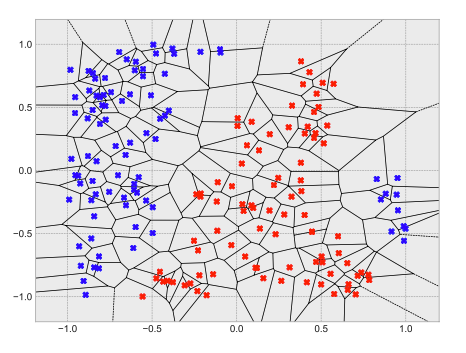
\includegraphics[width=0.6\columnwidth]{knn.png}
\end{center}

This method does not need any training and classification is done during test time. For a given training set $D$ it works as follows:
\begin{enumerate}
	\item Pick $k$ and distance metric $d$
	\item For given $x$, find among $x_1,...,x_n \in D$ the $k$ closest to $x \to x_{i_1},..., x_{i_k}$
	\item Output the majority vote of labels $y_{i_1},..., y_{i_k}$
\end{enumerate}

This method is very sensitive to $k$ and becomes unstable in high dimensions. We might need large $n$ for good results but computation can be reduces when allowing for some error probability.

\subsection{Decision Trees}

\begin{center}
	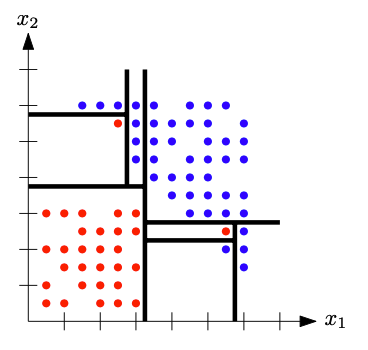
\includegraphics[width=0.52\columnwidth]{decision-tree}
\end{center}

A decision tree returns a partition of $X$ with sets aligned with the main axis. A given $x$ is assigned the majority class of the partition it lands in. The partitions can be modelled as leaf nodes of a binary tree. Single trees can easily overfit to noise, we have to choose the depth of the tree carefully.
\section{Neural Networks}

Success in learning crucially depends on the quality of the features. The key idea of neural networks is to parameterize the feature maps and optimize over the parameters.

We want to build a complex model out of simple components:
$$\phi(x, \theta) = \varphi(\theta^\top x)$$

Hereby, $\theta \in \R^d$ are the weights and $\varphi: \R \mapsto \R$ is a nonlinear \textbf{activation function}. Possible activation functions are:
\begin{itemize}
	\item \textbf{Identity}: $\varphi(z) = z$
	\item \textbf{Sigmoid}: $\varphi(z) = \frac{1}{1 + \exp(-z)}$
	\item \textbf{Tanh}: $\varphi(z) = \tanh z = \frac{\exp(z) - \exp(-z)}{\exp(z) + \exp(-z)}$
	\item \textbf{ReLU}: $\varphi(z) = \max (0,z)$
\end{itemize}

Nesting these components we create networks of the form:

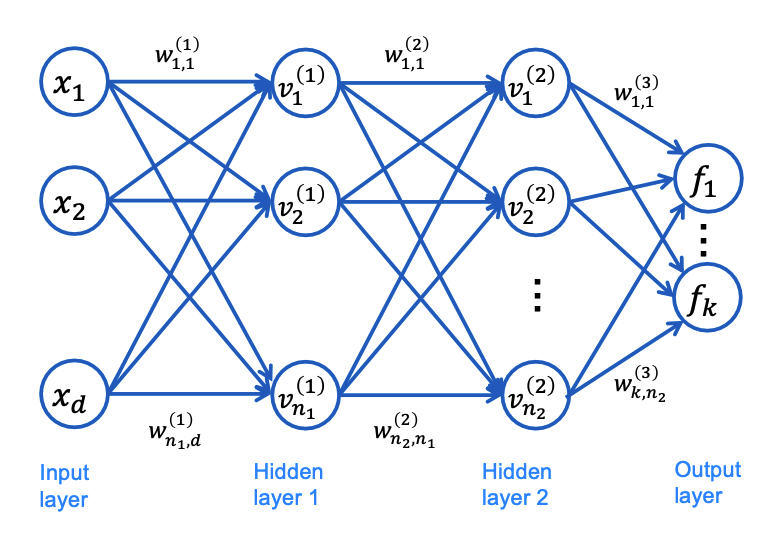
\includegraphics[width=\columnwidth]{neural-network.png}

Where $v_i = \varphi(z_i)$ and $z_i$ is the sum of inputs times their weight. To deal with biases we introduce a "constant" 1 feature to each layer. Note that we can have as many layers as we want and use different activation functions per layer. Such networks are typically trained via SGD.

By the universal approximation theorem, we can approximate any arbitrary smooth target function, given at least one layer with sufficient width.

\subsection{Forward Propagation}

This is the process of calculating the output for a given input.
\begin{itemize}
	\item For input layer 
		  $$v^{(0)} = [x; 1]$$
	\item For each hidden layer $1:L-1$
		  $$z^{(l)} = W^{(l)} v^{(l-1)} \quad \text{ and } \quad v^{(l)} = [\varphi(z^{(l)}); 1]$$
	\item For output layer
		  $$f = W^{(L)} v^{(L-1)}$$
\end{itemize}

\subsection{Backpropagation}

We can use the loss functions we already know to compute the loss. For multi output networks, we use the sum of per-output for regression tasks and cross-entropy loss for classification tasks. As mentioned we use SGD to fit our neural network. We want to jointly optimize over all weight for all layers. This is generally a non-convex optimization problem. Nevertheless, we can try to find a local optimum. In order to apply SGD, need to compute $\nabla_W \ell(W; x, y)$ w.r.t. each weight $w_{i,j}^{(l)}$:

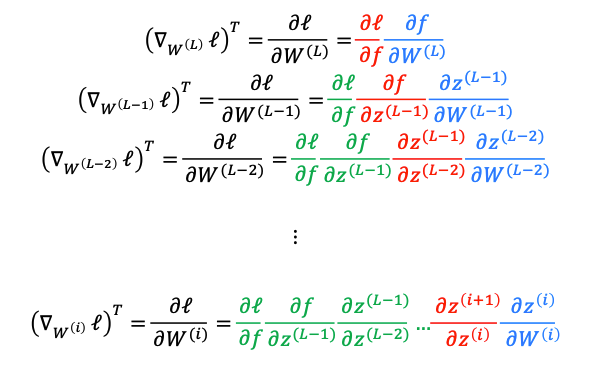
\includegraphics[width=\columnwidth]{backpropagation.png}

Notice that we can reuse calculations from \color{ForestGreen} \textbf{the previous layer} \color{Black}, \color{ProcessBlue} \textbf{forwards pass} \color{Black} and only have to compute \color{Red} \textbf{the gradient} \color{Black} for each layer.

Since the optimization problem is non-convex the initialization of the weights matters. With inappropriate weights we can run into exploding or vanishing gradients. To avoid this we randomly initialize the weights based on some distribution assumption for the activation function.

\subsection{Overfitting}

Since any deep neural network has a lot more parameters then data points to train on, overfitting can happen easily. To avoid this we use:
\begin{itemize}
	\item \textbf{Regularization}: add a penalty on the weights to the cost function
	\item \textbf{Early Stopping}: stop training once validation error stop to decrease
	\item \textbf{Dropout}: randomly ignore hidden units during training with probability $p$, after training all units are used and weights are multiplied by $p$
	\item \textbf{Batch Normalization}: normalize the input data (mean 0, variance 1) in each layer
\end{itemize}

\subsection{Convolutional Neural Networks}

CNN are a specialized architecture for neural networks. The idea is that predictions should be unchanged under some transformations of the data, e.g. rotation of images.

\begin{center}
	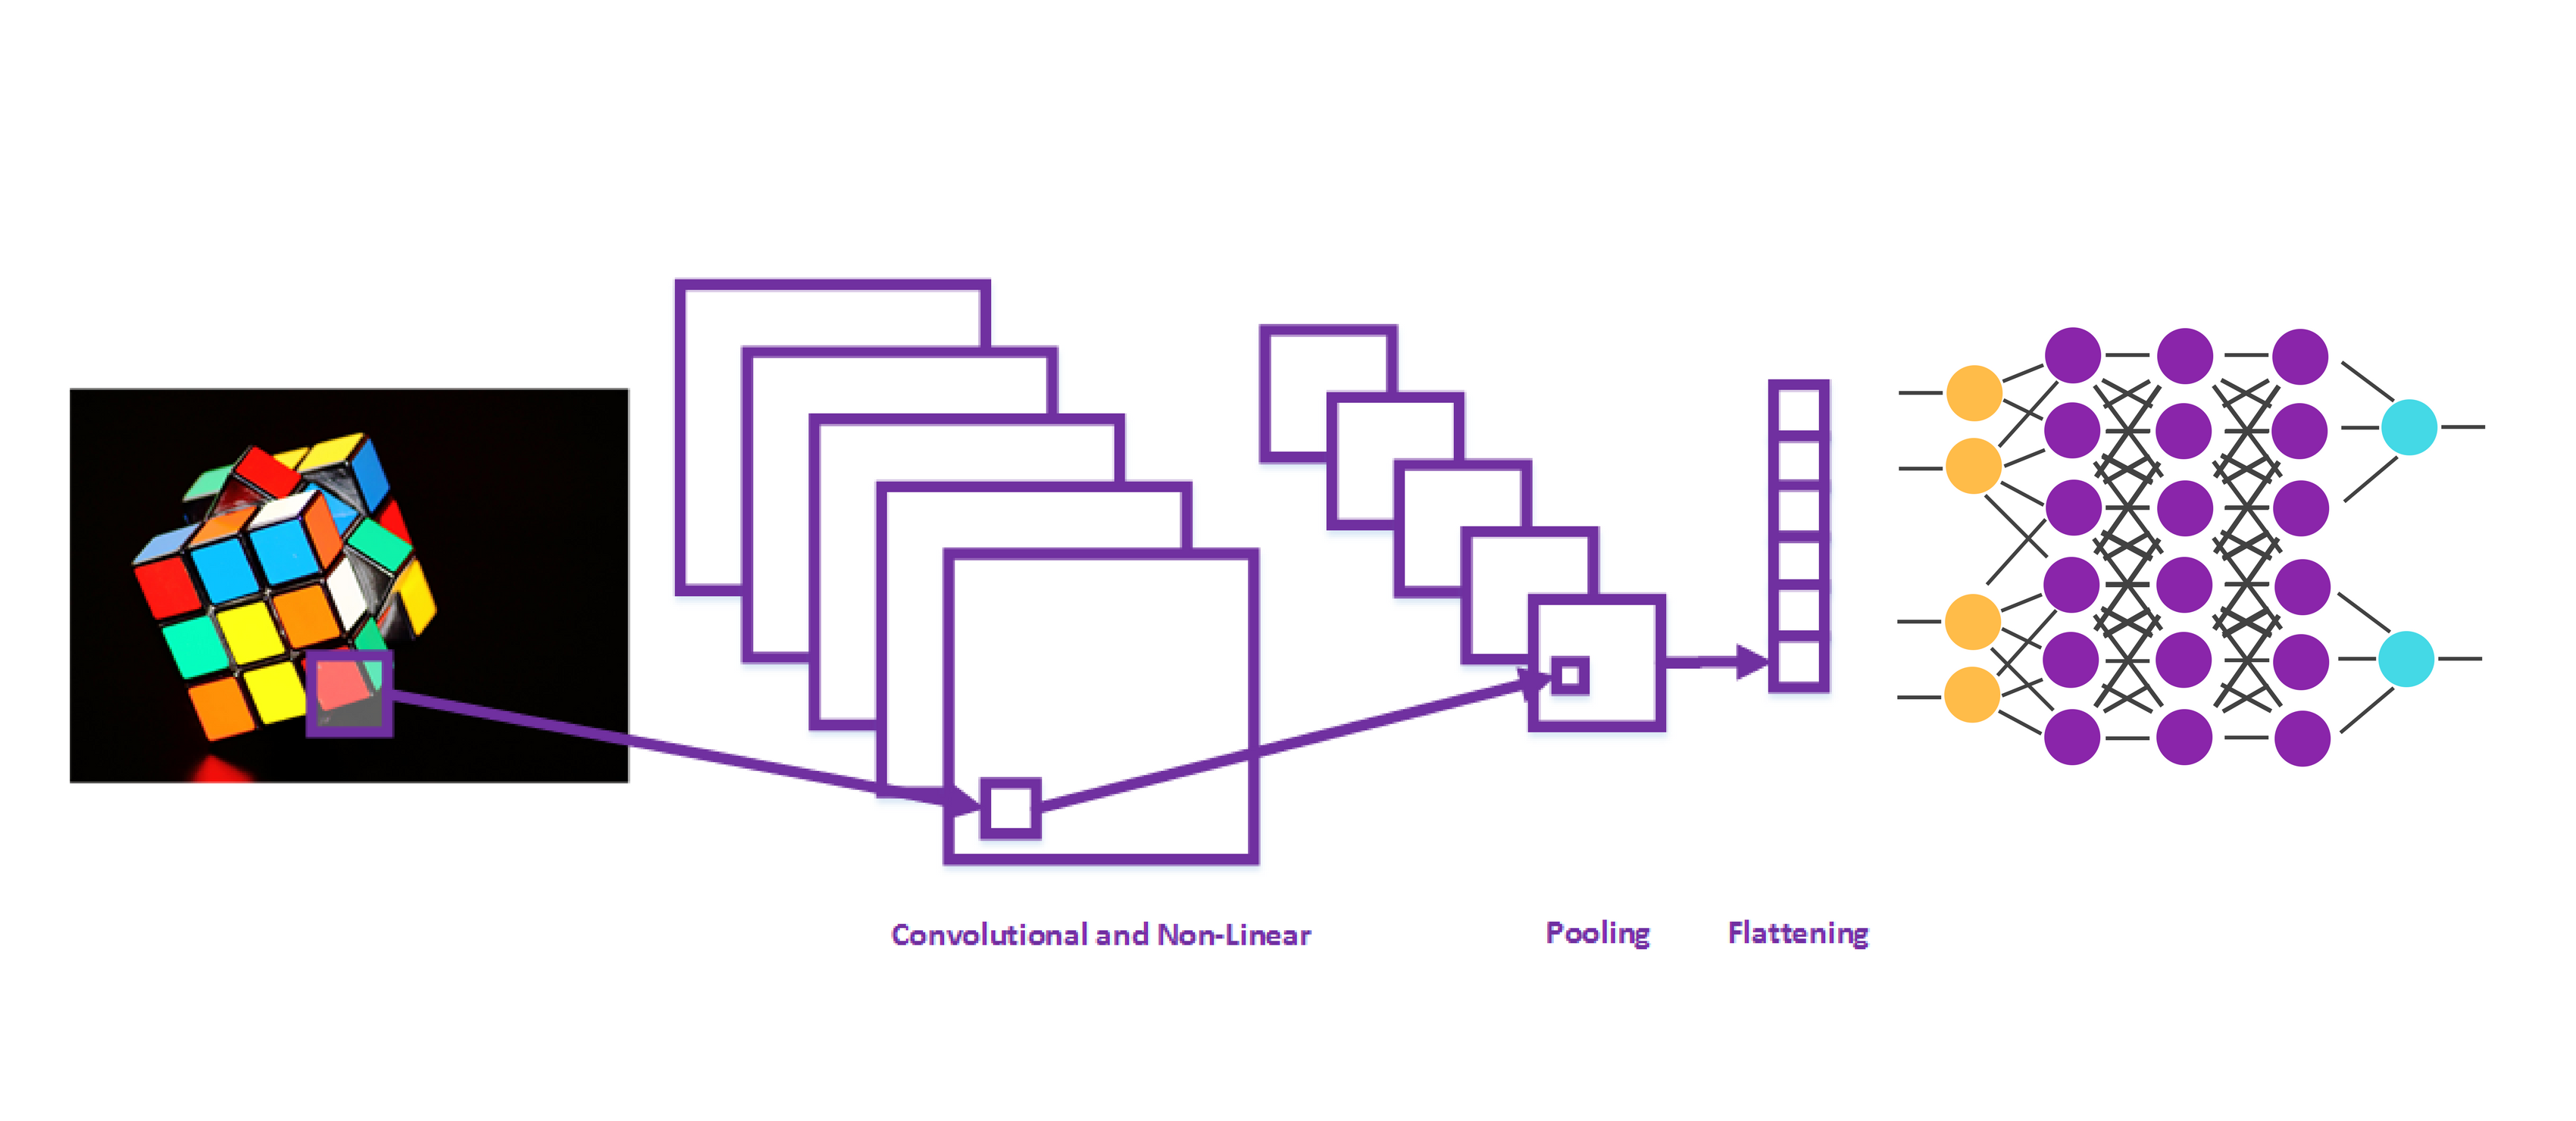
\includegraphics[width=\columnwidth]{cnn.png}
\end{center}

Each layer is not fully connected but structured. The activation function is applied to the element-wise convolution:
$$\varphi(W * v^{(l)})$$

The output dimension when applying $m$ different $f \times f$ filters to an $n \times n$ image with padding $p$ and stride $s$ is:
$$l = \frac{n + 2p - f}{s} + 1$$

Additionally we might use average or max pooling layers to aggregate several units into a single one, or use stride layers to skip units to decrease size.

\begin{center}
	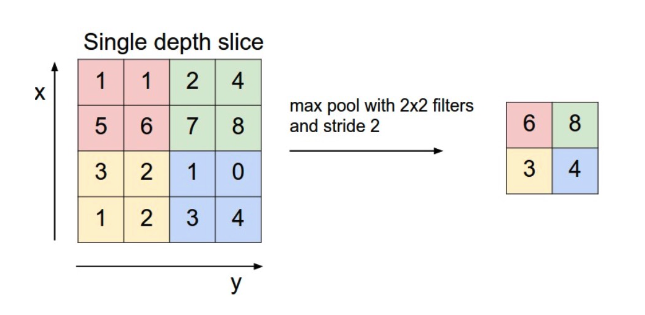
\includegraphics[width=\columnwidth]{pooling.png}
\end{center}


\section{Unsupervised Learning}

\subsection{k-Means Clustering}

Given an unlabelled dataset, we try to learn feature similarities based on proximity in feature space. Data points with similar features then should be grouped into the same cluster. k-Means tries to represent each cluster by a single (center) point $\mu_i$.

\begin{center}
	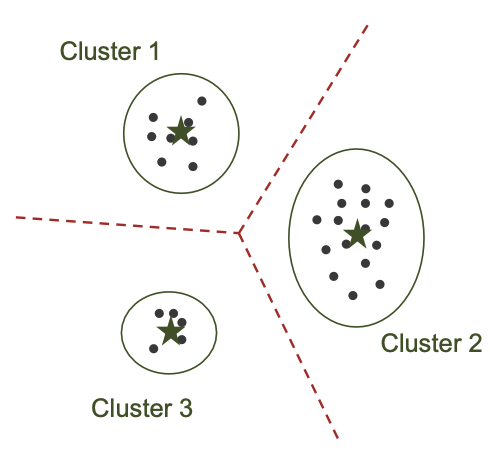
\includegraphics[width=0.6\columnwidth]{k-means.png}
\end{center}

Each data points is assigned by:
$$z_j = \argmin{i} ||x_j - \mu_i||_2, \quad z_j \in \{1, ..., k\}$$

To pick the optimal centers we try to minimize the sum of squared distances:
$$\hat{R} (\mu) = \sum_{i=1}^n \min_{j\in \{1,...,k\}} ||x_i - \mu_j||_2^2$$

This is a non-convex optimization problem and NP-hard. 

\columnbreak

One way of finding a good solution is Lloyd's heuristics:
\begin{enumerate}
	\item Initialize cluster centers $\mu^{(0)}$
	\item While not converged:
		\begin{enumerate}
			\item Assign each point to closest center:
				$$z_i \leftarrow \argmin{j\in \{1,...,k\}} ||x_i - \mu_j^{(t-1)}||_2$$		
			\item Update centers as mean of assigned data points:
				$$\mu_j^{(t)} \leftarrow \frac{1}{n_j} \sum_{i | z_i = j} x_i$$  	
		\end{enumerate}
\end{enumerate}

This guarantees to monotonically decrease the average squared distance in each iteration and converges to a local optimum. This local optimum is strongly dependent on the initialization. One way to initialize the centers is \textbf{k-Means++}:

\begin{enumerate}
	\item Start with random data point as center $\mu_1 = x_i$ where $i \sim \text{Unif}\{1,...,n\}$
	\item Add centers $2,...,k$ randomly, proportionally to the squared distance to closest selected center:
		$$\text{given } \mu_{1:j} \text{ pick } \mu_{j+1} = x_i$$ $$\text{ where } p(i) = \frac{1}{z} \min_{l \in \{1,...,j\}} ||x_i - \mu_l||_2^2$$
\end{enumerate}

To find the optimal number of clusters $k$ can not be done by cross-validation, as the loss keeps decreasing with larger $k$. We can either keep increasing $k$ until we reach a negligible decrease in loss or we can use regularization to add a penalty term for larger $k$.

\subsection{Principal Component Analysis}

PCA is used for dimensionality reduction. Given data $x_i \in \R^d$ we want to obtain a low-dimensional representation $z_i \in \R^k$ where $k < d$. One of the benefits of low-dimensional representation is that we can visualize data that we otherwise could not. Feature discovery is another use case for PCA, it can help us to discover features from data, e.g. Eigenfaces. We assume that our data is centered around the origin. 

Our goal is to learn the function $f(x) = Ax$ that maps the high dimensional data to the lower dimensions, while minimizing the reconstruction error. First we will look at the case $k = 1$.
$$\min_{w, z} \sum_{i=1}^n ||x_i - z_i w||_2^2 \quad \text{s.t. } ||w||_2 = 1$$

We limit $w$ to be of unit length to guarantee a unique solution.

\begin{center}
	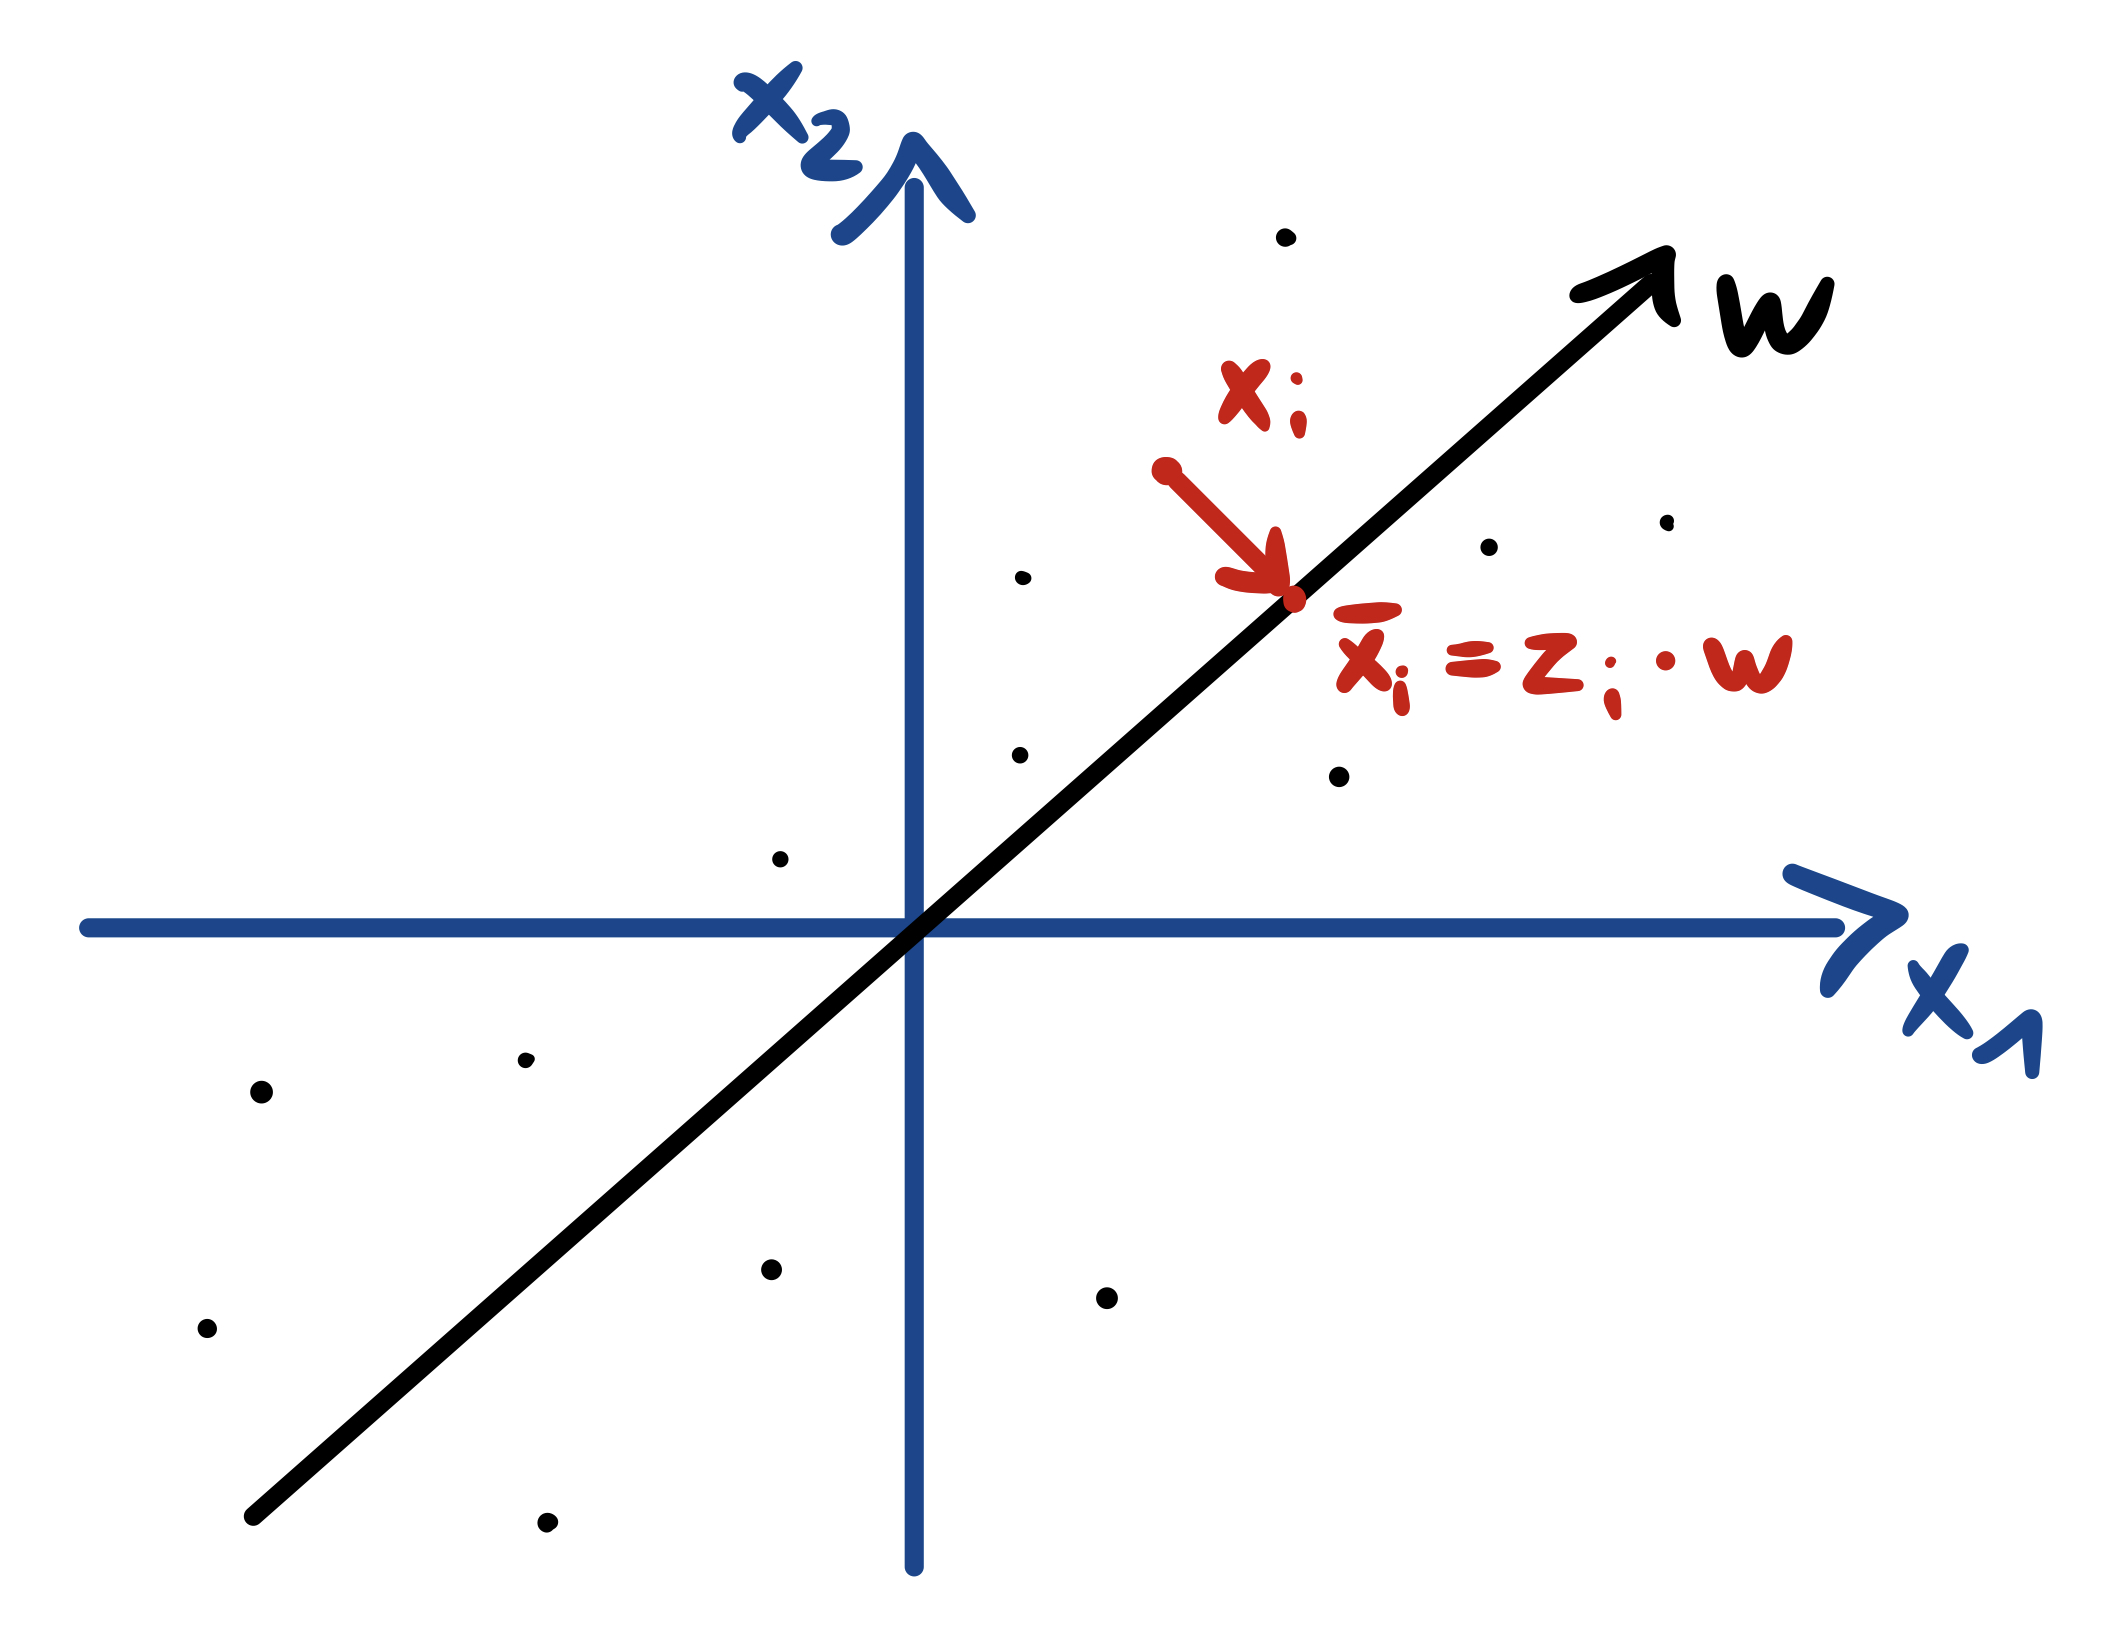
\includegraphics[width=0.7\linewidth]{pca.jpeg}
\end{center}

Since for a given $w$ the minimal distance vector $\bar{x}_i - x_i$ is perpendicular to $w$, we find that the optimal solution for $z_i = w^\top x_i$. We can now substitute $z_i$ and receive the following optimization goal:
$$\hat{w} = \argmin{||w||_2=1} \sum_{i=1}^n ||x_i - w w^\top x_i||_2^2$$

Which again can be reformulated as:
$$\hat{w} = \argmax{||w||_2=1} \; \sum_{i=1}^n (w^\top x_i)^2 \text{ or } \hat{w} = \argmax{||w||_2=1} \; w^\top \Sigma w$$

Where $\Sigma = \frac{1}{n} \sum_{i=1}^n x_i x_i^\top$ is the empirical covariance. Since we still have an argmax this is not a minimization problem anymore and we can not find a solution like in previous problems. There still exists a closed form solution given by the principal eigenvector of $\Sigma$, i.e. $w = v_1$ where for $\lambda_1 \geq ... \geq \lambda_d \geq 0$:
$$\Sigma = \sum_{i=1}^d \lambda_i v_i v_i^\top$$

Up until now everything was for $k = 1$. For $k > 1$ we have to change the normalization from $||w||_2 = 1$ to $W^\top W = I$ everything else is basically the same, we just take the first $k$ principal eigenvectors so that $W = [v_1, ..., v_k]$.

Choosing the optimal $k$ is different depending on our goal, for feature induction we use cross-validation else we often pick $k$ so that the variance of our data is mostly explained (other dimensions would add little information).

\subsubsection{PCA through SVD}

Another way of obtaining the PCA is through singular-value decomposition. Recall that we can represent any data matrix $X$ as $U S V^\top$ where $S$ is a diagonal matrix containing the singular values (singular values being the square root of eigenvalues). Now the top $k$ principal components are exactly the first $k$ columns of $V$.

\subsubsection{Kernel PCA}

Again we run into problems trying to work with complex arrangements of data, e.g. circles, swiss roll, etc.

\begin{center}
	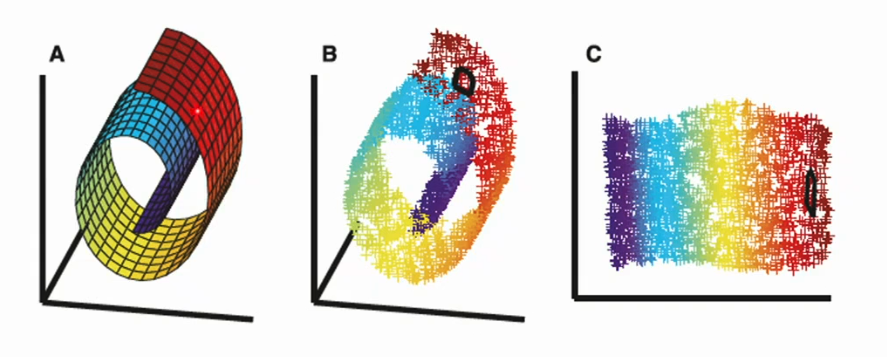
\includegraphics[width=\linewidth]{swiss-roll.png}
\end{center}

Similar to supervised learning where we worked with kernels, we can take the same approach for unsupervised learning. Since it holds $\Sigma = \frac{1}{n} \sum_{i=1}^n x_i x_i^\top = X^\top X$ we can apply the kernel trick. We start by assuming $w = \Phi^\top \alpha$, plugging this into our objective and the constraint we end up with:
$$\hat{\alpha} = \argmax{\alpha} \; \frac{\alpha^\top K^\top K \alpha}{\alpha^\top K \alpha}$$

We arrive at the general closed form solution:
$$\alpha^{(i)} = \frac{1}{\sqrt{\lambda_i}}v_i \quad K = \sum_{i = 1}^n \lambda_i v_i v_i^\top \quad \lambda_1 \geq ... \geq \lambda_n \geq 0$$

Given this, a new point $x$ is projected as $z$ where:
$$z_i = \sum_{j=1}^n \alpha_j^{(i)} k(x_j, x)$$

\subsection{Autoencoders}

Autoencoders are neural networks with a bottleneck layer and $d_{in} = d_{out}$. We want to minimize $\frac{1}{n}\sum_{i=1}^n ||x_i - \hat{x}_i||_2^2$. The idea is to learn the identity function:
$$\hat{x} = f(x; \theta) \text{ where } f(x; \theta) = f_{dec}(f_{enc}(x, \theta_{enc}); \theta_{dec})$$

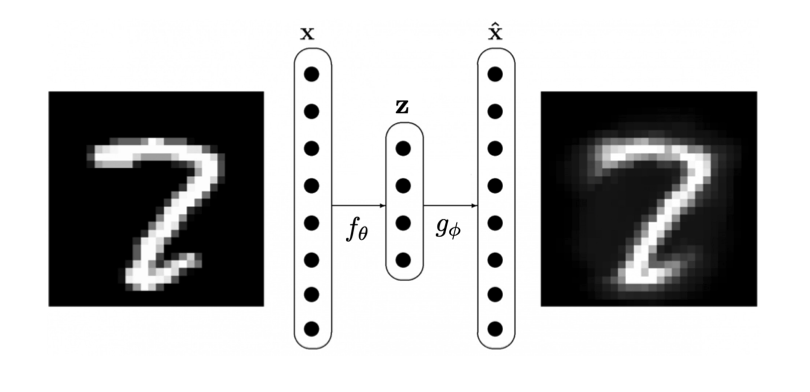
\includegraphics[width=\linewidth]{autoencoder.png}

If linear activation functions and the square loss between input and output are used, then the encoder learns PCA. Otherwise it learns some nonlinear embedding $z$ of the features.
\section{Statistical Perspective}

In this part we will explore a statistical perspective on supervised learning by estimating the data distribution and then deriving a decision rule from the distribution. This allows us to express prior knowledge about the data. We start with the fundamental assumption that our data is generated iid. by some unknown distribution, note that this assumption is often violated in practice:
$$(x_i, y_i) \sim p(x, y)$$

We want to find a hypothesis $f: X \mapsto Y$ that minimizes the \textbf{expected loss / prediction error / population risk} (over all possible data):
$$R(f) = \int p(x,y) \ell(y, f(x)) dxdy = \E_{x,y}[\ell(y, f(x))]$$

We have already seen that the \textbf{empirical risk / training error} $\hat{R}_D(f)$ often underestimates the population risk. But by the law of large numbers we have that empirical risk approaches the population risk. We call this difference $|\hat{R}_D(f) - R(f)|$ the \textbf{generalization error} w.r.t. $f$.

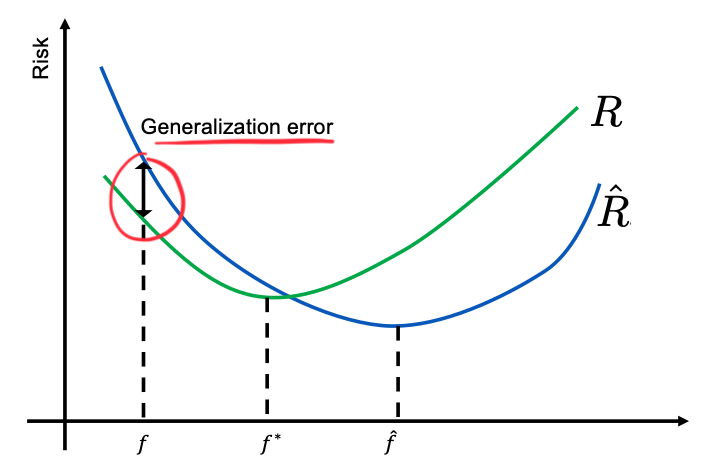
\includegraphics[width=\columnwidth]{risk.png}

\subsection{Optimal Predictor for the Squared Loss}

The population risk for the squared loss is:
$$R(f) = \E_{x,y}[(y - f(x))^2]$$

Suppose we knew $p(x,y)$ which $f$ minimizes the population risk?
\begin{align*}
	f^* &= \min_f \E_{x,y}[(y - f(x))^2] \\
	&= \min_f \E_x[\E_y[(y - f(x))^2 \; | \; X=x]] \\
	&= \E_x[ \min_f \E_y[(y - f(x))^2 \; | \; X=x]]
\end{align*}

Now we focus on the inner part, suppose we are given a fixed $x$:
$$f^*(x) = \argmin{\hat{y}} \; \E_y[(\hat{y} - y)^2 \; | \; X = x)] = \E[y \; | \; X = x]$$

We therefore have shown that $f^*$ minimizing the population risk is given by the conditional mean, which can be calculated by:
$$f^*(x) = \E[y \; | \; X = x] = \int y \cdot p(y \; | \; x) dy$$

Note that we only need the conditional distribution $p(y \; | \; x)$ and not the full joint distribution $p(x, y)$. Thus one strategy is for estimating a predictor from training data is to estimate the conditional distribution $\hat{p}(y \; | \; x)$ and then use it to predict labels via the conditional mean. \medskip

One common approach to estimate the conditional distribution is to choose a particular parametric form and then estimate the parameters $\theta$ with the maximum (log) likelihood estimation:
\begin{align*}
	\theta^* &= \argmax{\theta} \; \hat{p}(y_1, ..., y_n \; | \; x_1, ..., x_n, \theta) \\
	&= \argmin{\theta} \; - \sum_{i=1}^n \log p(y_i \; | \; x, \theta) 
\end{align*}

\subsubsection{Example: Conditional Linear Gaussian}

Let us look at the case where we make the assumption that the noise is Gaussian. We have $y = f(x) + \epsilon$ with $\epsilon \sim \mathcal{N}(0, \sigma^2)$ and $f(x) = w^\top x$. Therefore the conditional probability is:
\begin{center}
	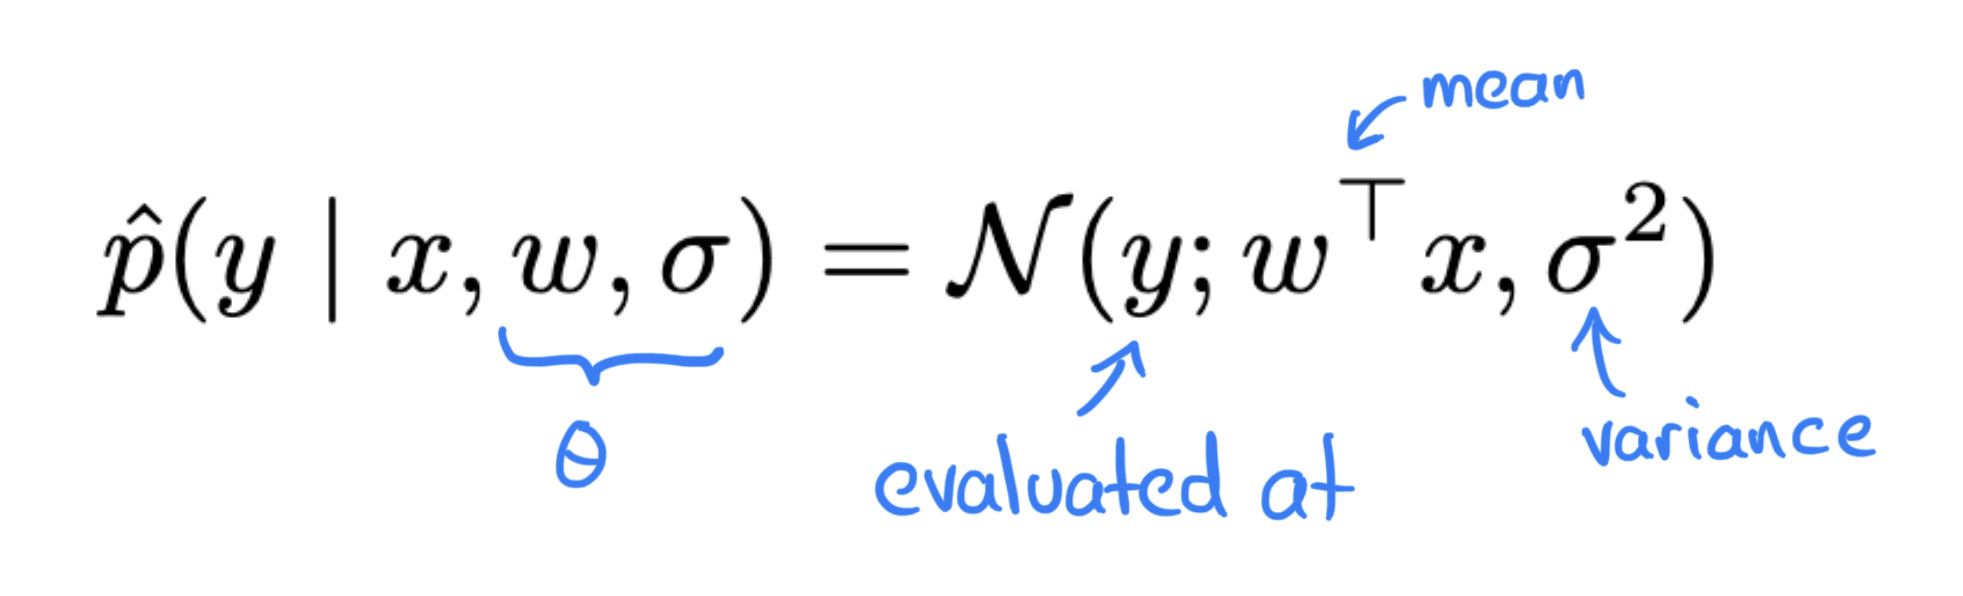
\includegraphics[width=0.7\columnwidth]{gaussian-conditional-prob.jpeg}
\end{center}

Then we can find the optimal $\hat w$ by using the definition of the normal distribution (some steps are left out):
\begin{align*}
	\hat w &= \argmax{w} \; \hat p(y_{1:n} \; | \; x_{1:n}, w, \sigma) \\
	&= \argmin{w} \sum_{i=1}^n - \log \mathcal{N}(y_i \; | \; x_i, w^\top x, \sigma^2) \\
	&= \argmin{w} \sum_{i=1}^n (y_i - w^\top x_i)^2
\end{align*}

Therefore we have shown that under the conditional linear Gaussian assumption, the MLE is equivalent to the least squares estimation.

\subsubsection{Bias-Variance Tradeoff}

Recall that the following hold:
$$\text{Prediction Error} = \text{Bias}^2 + \text{Variance} + \text{Noise}$$

Where we have:
\begin{itemize}
	\item \textbf{Bias}: Excess risk of best model considered compared to minimal achievable risk knowing $p(x,y)$
	\item \textbf{Variance}: Risk incurred due to estimating model from limited data
	\item \textbf{Noise}: Risk incurred by optimal model (irreducible error)
\end{itemize}

The MLE for linear regression is unbiased, further it is the minimum variance estimator among all unbiased estimators. However, we have also seen that it can overfit.

\subsection{Maximum a Posteriori Estimate}

It is often favourable to introduce some bias (make assumptions) to reduce variance drastically. One such assumption could be that the weights are small. We can capture this assumption with a Gaussian prior $w_i \sim \mathcal{N}(0, \beta^2)$. Then, the posterior distribution of $w$ is given by:
\begin{align*}
	p(w \; | \; \bar x, \bar y) &= \frac{p(w, \bar x, \bar y)}{p(\bar x, \bar y)} \\
	&= \frac{p(w, \bar y \; | \; \bar x) \cdot p(\bar x)}{p(\bar y \; | \; \bar x) \cdot p(\bar x)} \\
	&= \frac{p(w) \cdot p(\bar y \; | \; w, \bar x)}{p(\bar y \; | \; \bar x)}
\end{align*}

Hereby we used that $w$ is apriori independent of $\bar x$ (note that $\bar x = x_{1:n}, \bar y = y_{1:n}$). Now we want to find the maximum a posteriori estimate (MAP) for $w$:
\begin{align*}
	\hat w &= \argmax{w} \; p(w \; | \; \bar x, \bar y) \\
	&= \argmin{w} \; - \log p(w) - \log p(\bar y \; | \; w, \bar x) + \log p(\bar y \; | \; \bar x) \\
	&= \argmin{w} \; \frac{\sigma^2}{\beta^2} ||w||_2^2 + \sum_{i=1}^n(y_i - w^\top x_i)^2
\end{align*}

Which is exactly the same as ridge regression with $\lambda = \frac{\sigma^2}{\beta^2}$. More generally, regularized estimation can often be understood as MAP inference, with different priors (= regularizers) and likelihoods (= loss functions).

\subsection{Statistical Models for Classification}

We now want to do the same risk minimization for classification. The population risk for the 0-1 loss is:
$$R(f) = \mathbb P[y \neq f(x)] = \E_{x,y}[\mathbb I_{y \neq f(x)}]$$

Suppose we knew $p(x,y)$ which $f$ minimizes the population risk?
\begin{align*}
	f^*(x) &= \argmin{\hat y} \; \E_y [\mathbb I_{y \neq \hat y} \; | \; X = x] \\
	&= \argmax{\hat y} \; p(\hat y \; | \; x)
\end{align*}

This hypothesis $f^*$ minimizing the population risk is given by the most probable class, this hypothesis is called the Bayes' optimal predictor for the 0-1 loss.

Similar to the regression we can now look at logistic regression and assume that we have iid. Bernoulli noise. Therefore the conditional probability is:
$$p(y \; | \; x,w) \sim \text{Ber}(y; \sigma(w^\top x))$$

Where $\sigma(z) = \frac{1}{1 + \exp(-z)}$ is the sigmoid function. Using MLE we get:
\begin{align*}
	\hat w &= \argmax{w} \; p(\bar y \; | \; w, \bar x) \\
	&= \argmin{w} \sum_{i = 1}^n \log (1 + \exp(-y_i w^\top x_i))
\end{align*}

Which is exactly the logistic loss. Instead of solving MLE we can estimate MAP, e.g. with a Gaussian prior:
\begin{align*}
	\hat w &= \argmax{w} \; p(w \; | \; \hat x, \hat y) \\
	&= \argmin{w} \; \lambda ||w||_2^2 + \sum_{i = 1}^n \log (1 + \exp(-y_i w^\top x_i))
\end{align*}







\section{Bayesian Decision}


\section{Generative Modeling}

In the previous part we looked at \textbf{discriminative models} with the aim to estimate the conditional distribution $p(y \; | \; x)$. Generative models aim to estimate the joint distribution $p(x, y)$. This will help us to model much more complex situations. Remember Bayes' rules:
$$p(y \; | \; x) = \frac{1}{z} \underbrace{p(y) \cdot p(x \; | \; y)}_{p(x,y)}$$

Where $z$ is the normalization constant $p(x)$. Generative modeling can be seen as the seen as the attempt to infer the process, according to which examples are generated.

\subsection{Naive Bayes Model}

We want to apply generative modeling for classification tasks. We starte by making the assumption that given some class label, each feature is independent of all the other features (therefore naive). This helps us estimating $p(\bar x \; | \; \bar y)$ as it is equal to $\prod_{i=1}^d p(x_i \; | \; y_i)$. \medskip

\subsection{Gaussian Naive Bayes Classifier}

We model the features by conditionally independent Gaussians and estimate the parameters via maximum likelihood estimation:
\begin{enumerate}
	\item MLE for class prior:
		$$p(y) = \hat p_y = \frac{\text{Count}(Y = y)}{n}$$
	\item MLE for feature distribution:
		$$p(x_i \; | \; y) = \mathcal{N}(x_i; \hat \mu_{y,i}), \sigma^2_{y,i}$$
\end{enumerate}

Where:
\begin{align*}
	\mu_{y,i} &= \frac{1}{\text{Count}(Y = y)} \sum_{j \; | \; y_j = y} x_{j,i}\\
	\sigma^2_{y,i} &= \frac{1}{\text{Count}(Y = y)} \sum_{j \; | \; y_j = y} (x_{j,i} - \hat \mu_{y, i})^2
\end{align*}

Predictions are then made by:
$$y = \argmax{\hat y} \; p(\hat y \; | \; x) = \argmax{\hat y} \; p(\hat y) \cdot \prod_{i=1}^d p(x_i \; | \; \hat y)$$

\begin{center}
	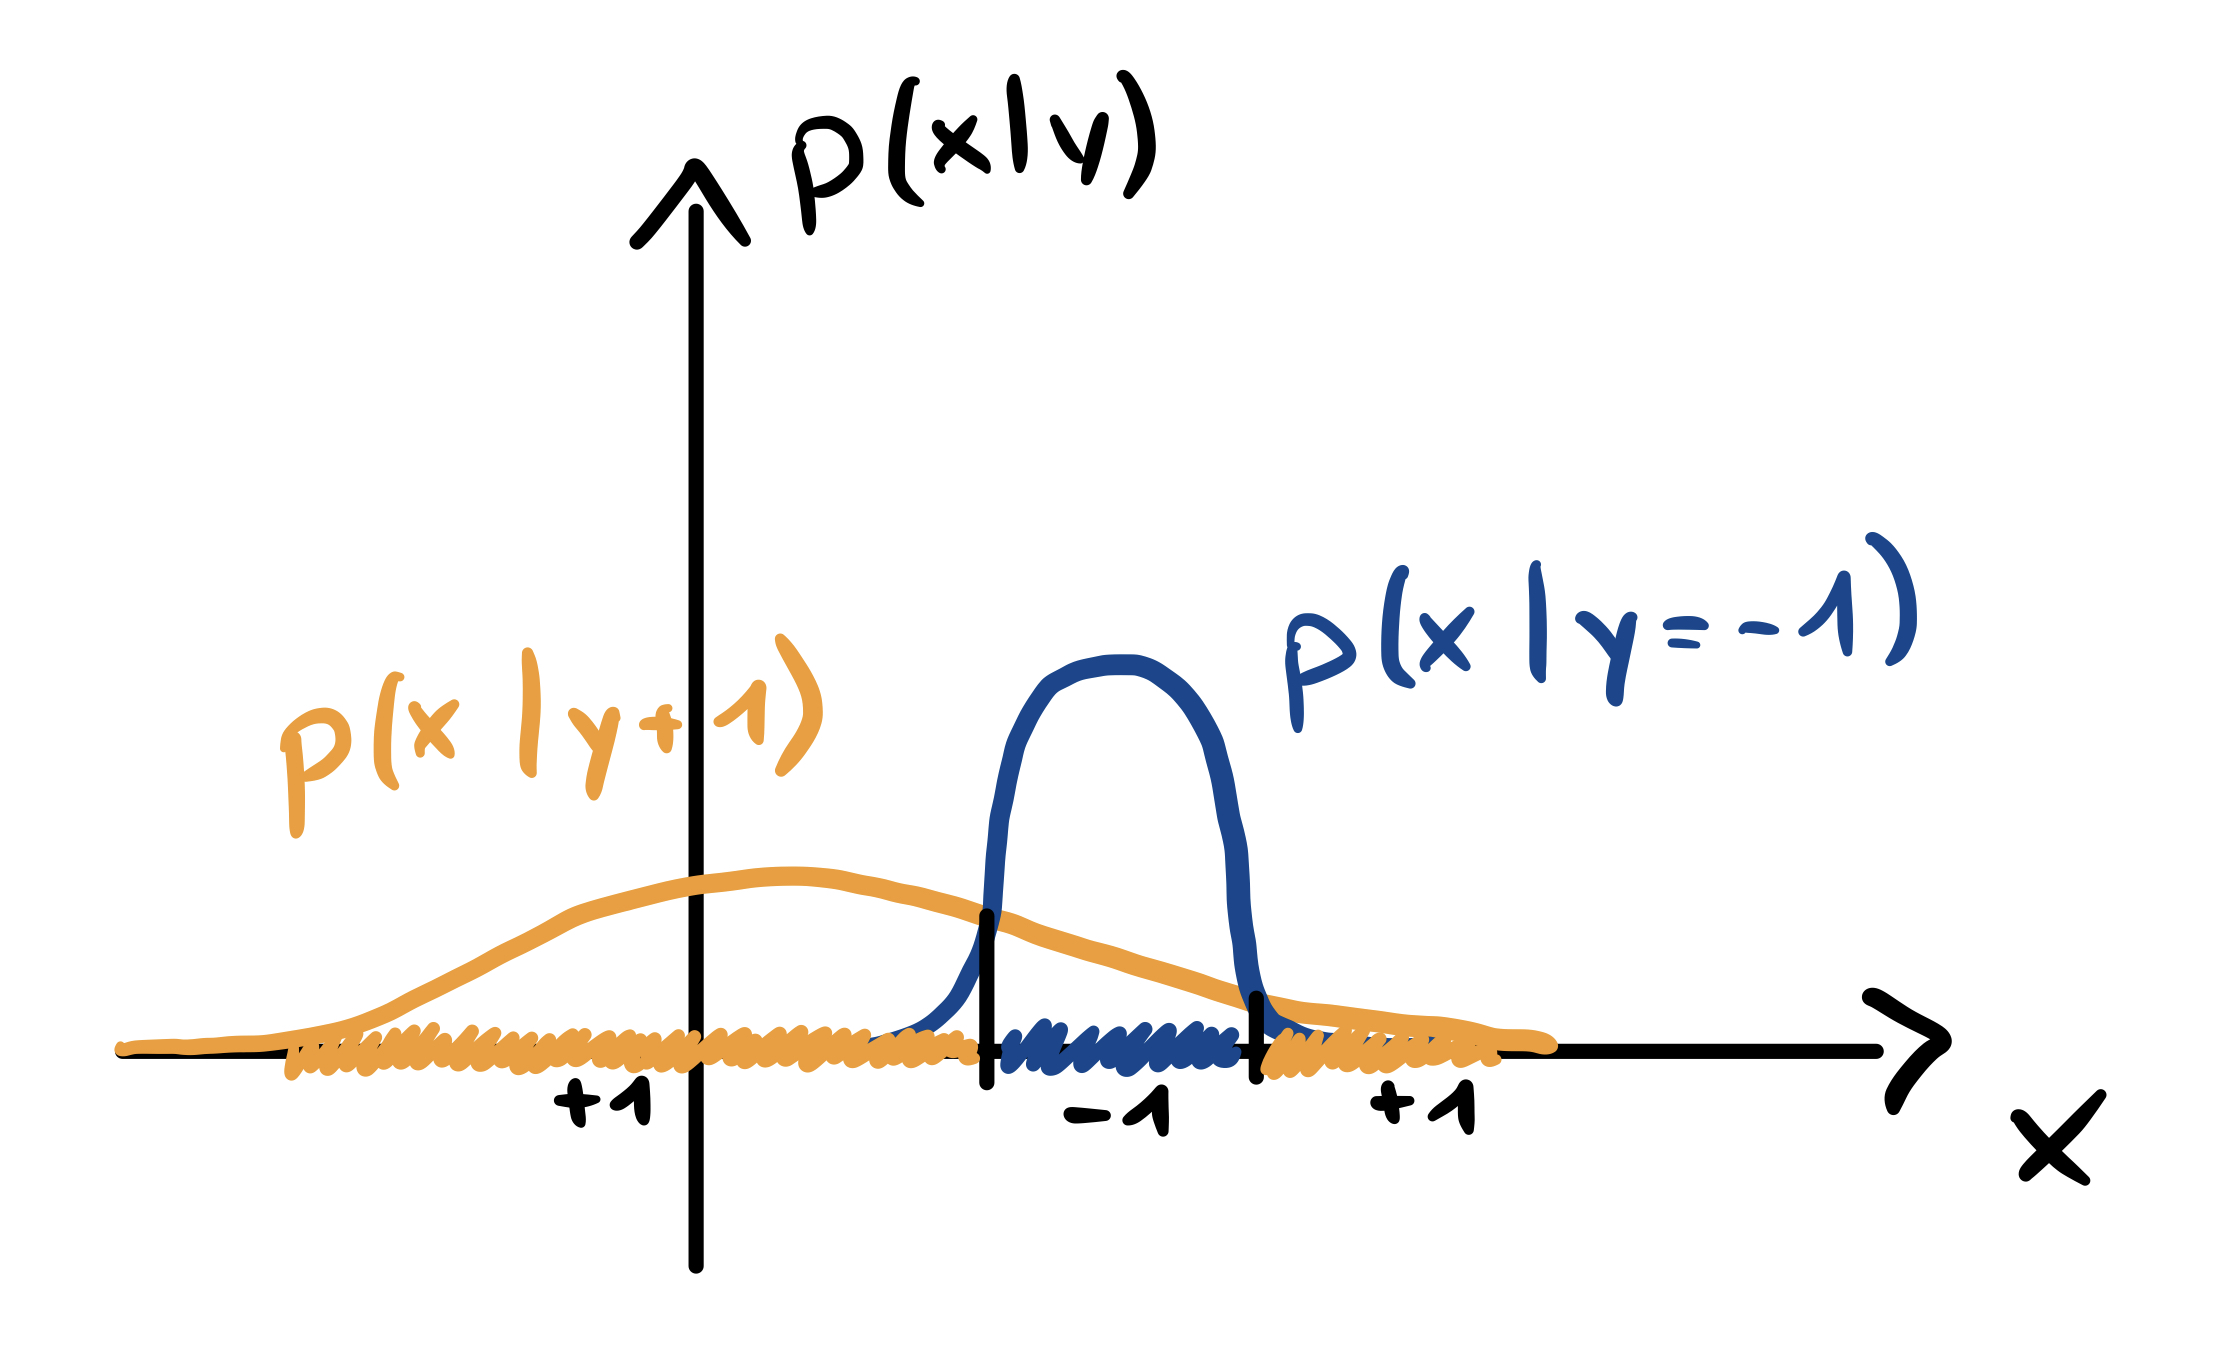
\includegraphics[width=0.8\columnwidth]{gnb.jpeg}
\end{center}

This is equivalent to the following decision rule for binary classification:
$$y = \sgn \underbrace{\left( \log \frac{p(Y = +1 \; | \; x)}{p(Y = -1 \; | \; x)} \right)}_{f(x)}$$

Where $f(x)$ is called the discriminant function. We can rewrite this and get:
\begin{align*}
f(x) &= \sum_{i=1}^d \underbrace{\frac{1}{\sigma_i^2} (\mu_{+1,i} - \mu_{-1,i})}_{w_i} \cdot x_i \\
&+ \underbrace{\log \frac{p}{1-p} + \sum_{i=1}^d \frac{1}{2 \sigma_i^2} (\mu_{-1, i}^2 - \mu_{+1, i}^2)}_{w_0}
\end{align*}

If the conditional independence assumption is violated, we can run into some serious issues, e.g. the classifier can become overconfident.

\subsection{Gaussian Bayes Classifier}

We drop the independence assumption and model our features as generated by a multivariant Gaussian $\mathcal{N}(x; \mu_y, \Sigma_y)$ with:
\begin{align*}
	\mu_{y} &= \frac{1}{\text{Count}(Y = y)} \sum_{j \; | \; y_j = y} x_{j}\\
	\Sigma_{y} &= \frac{1}{\text{Count}(Y = y)} \sum_{j \; | \; y_j = y} (x_{j} - \hat \mu_{y}) (x_{j} - \hat \mu_{y})^\top
\end{align*}

This is also called the \textbf{quadratic discriminant analysis} (QDA). 

\begin{center}
	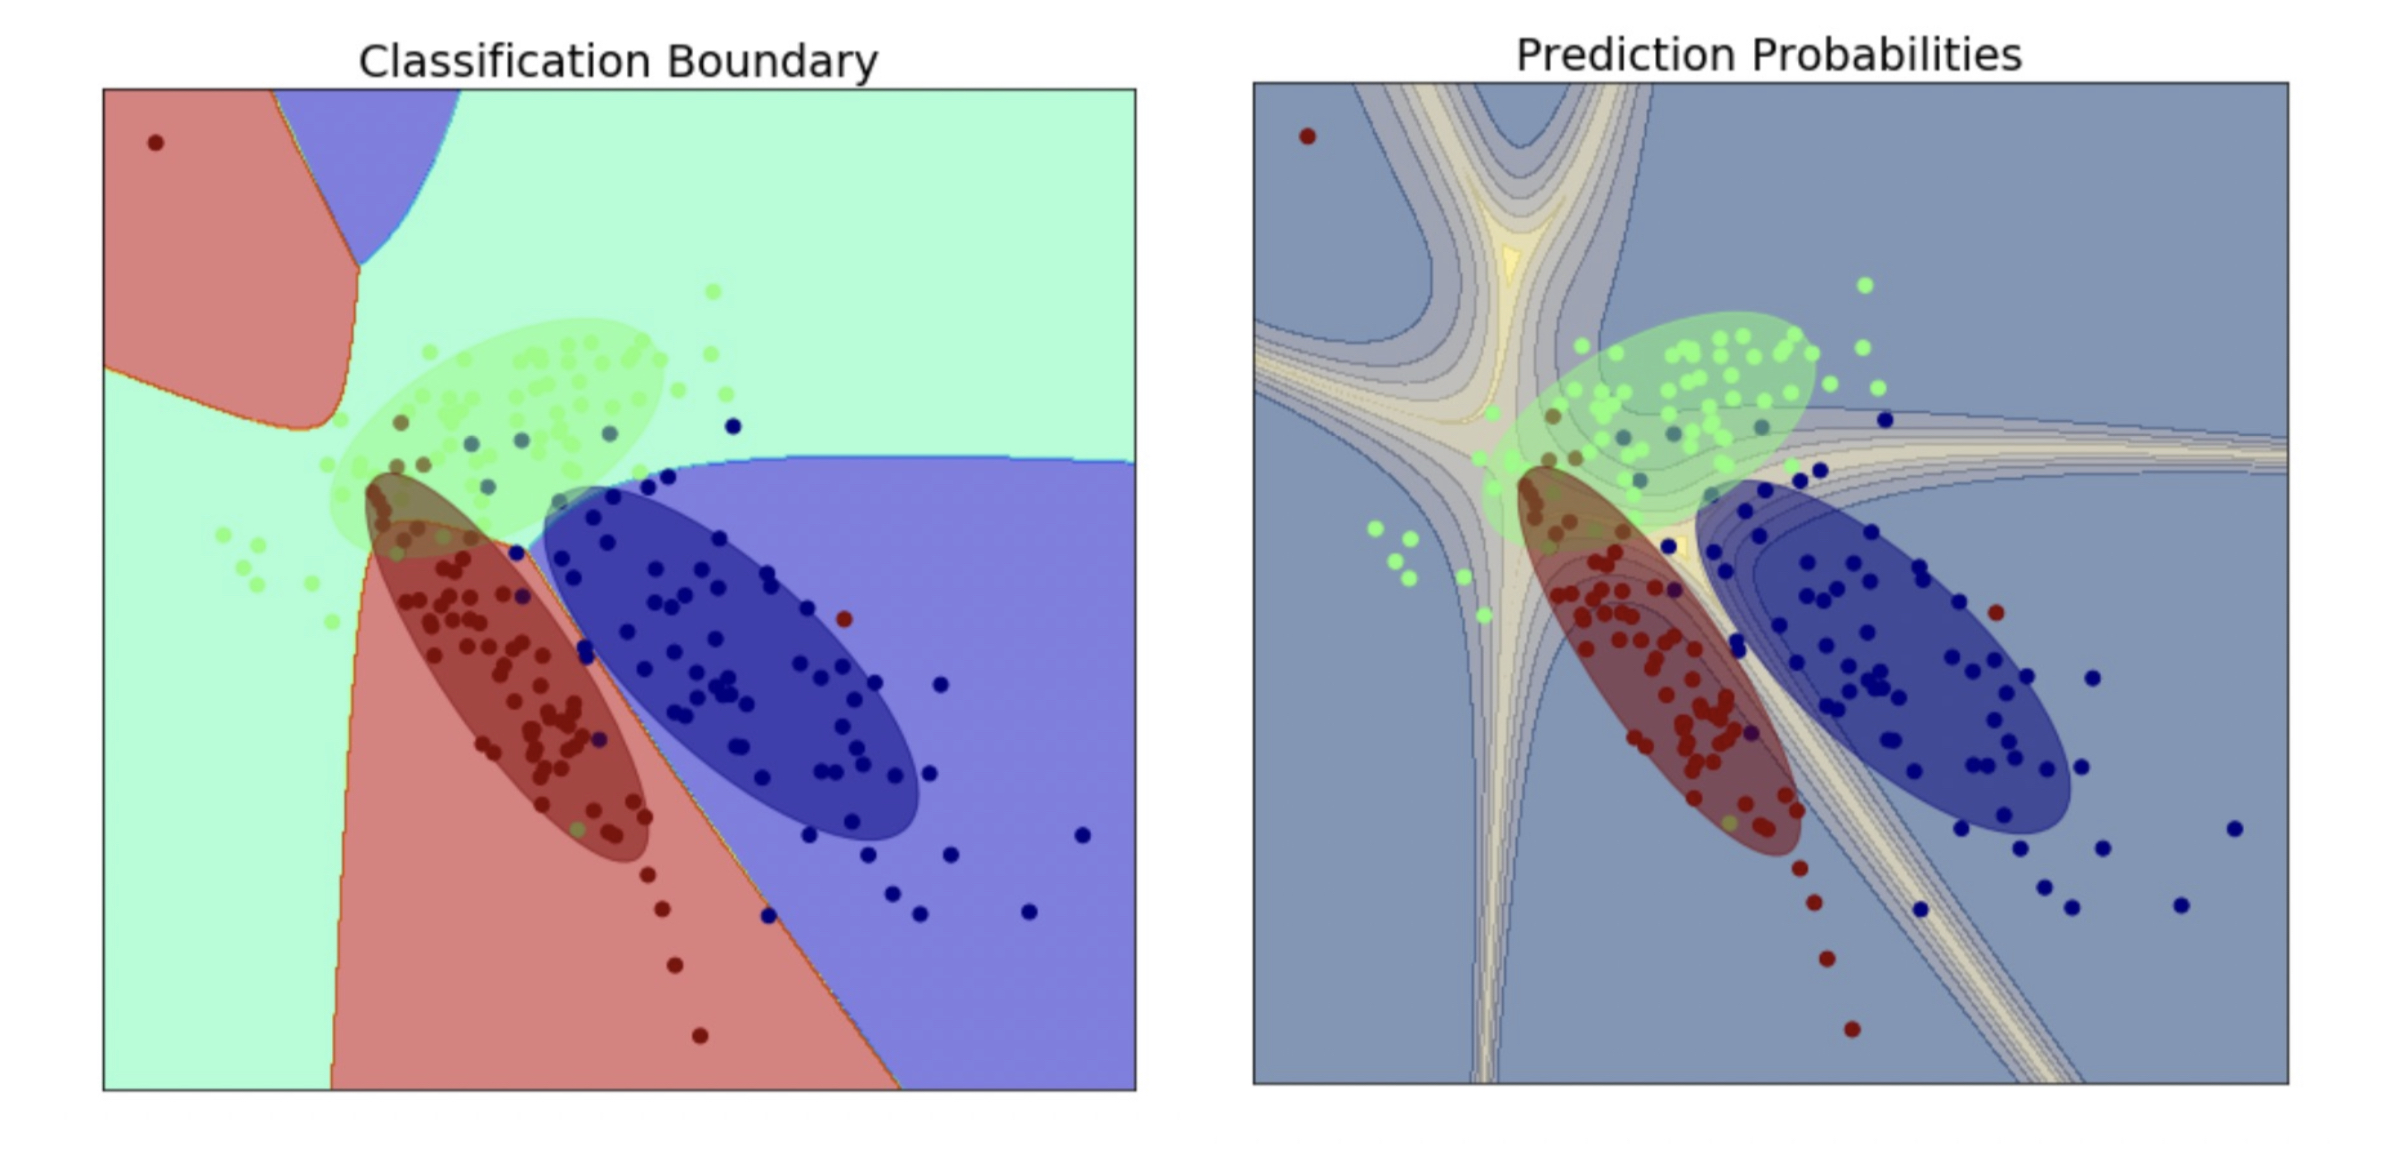
\includegraphics[width=\columnwidth]{qda.jpeg}
\end{center}

If we impose the restriction that $\Sigma_+ = \Sigma_-$ this leads us to the linear discriminant analysis LDA and if we further restrict $p(y) = \frac{1}{2}$ we get the Fisher LDA.

\begin{center}
	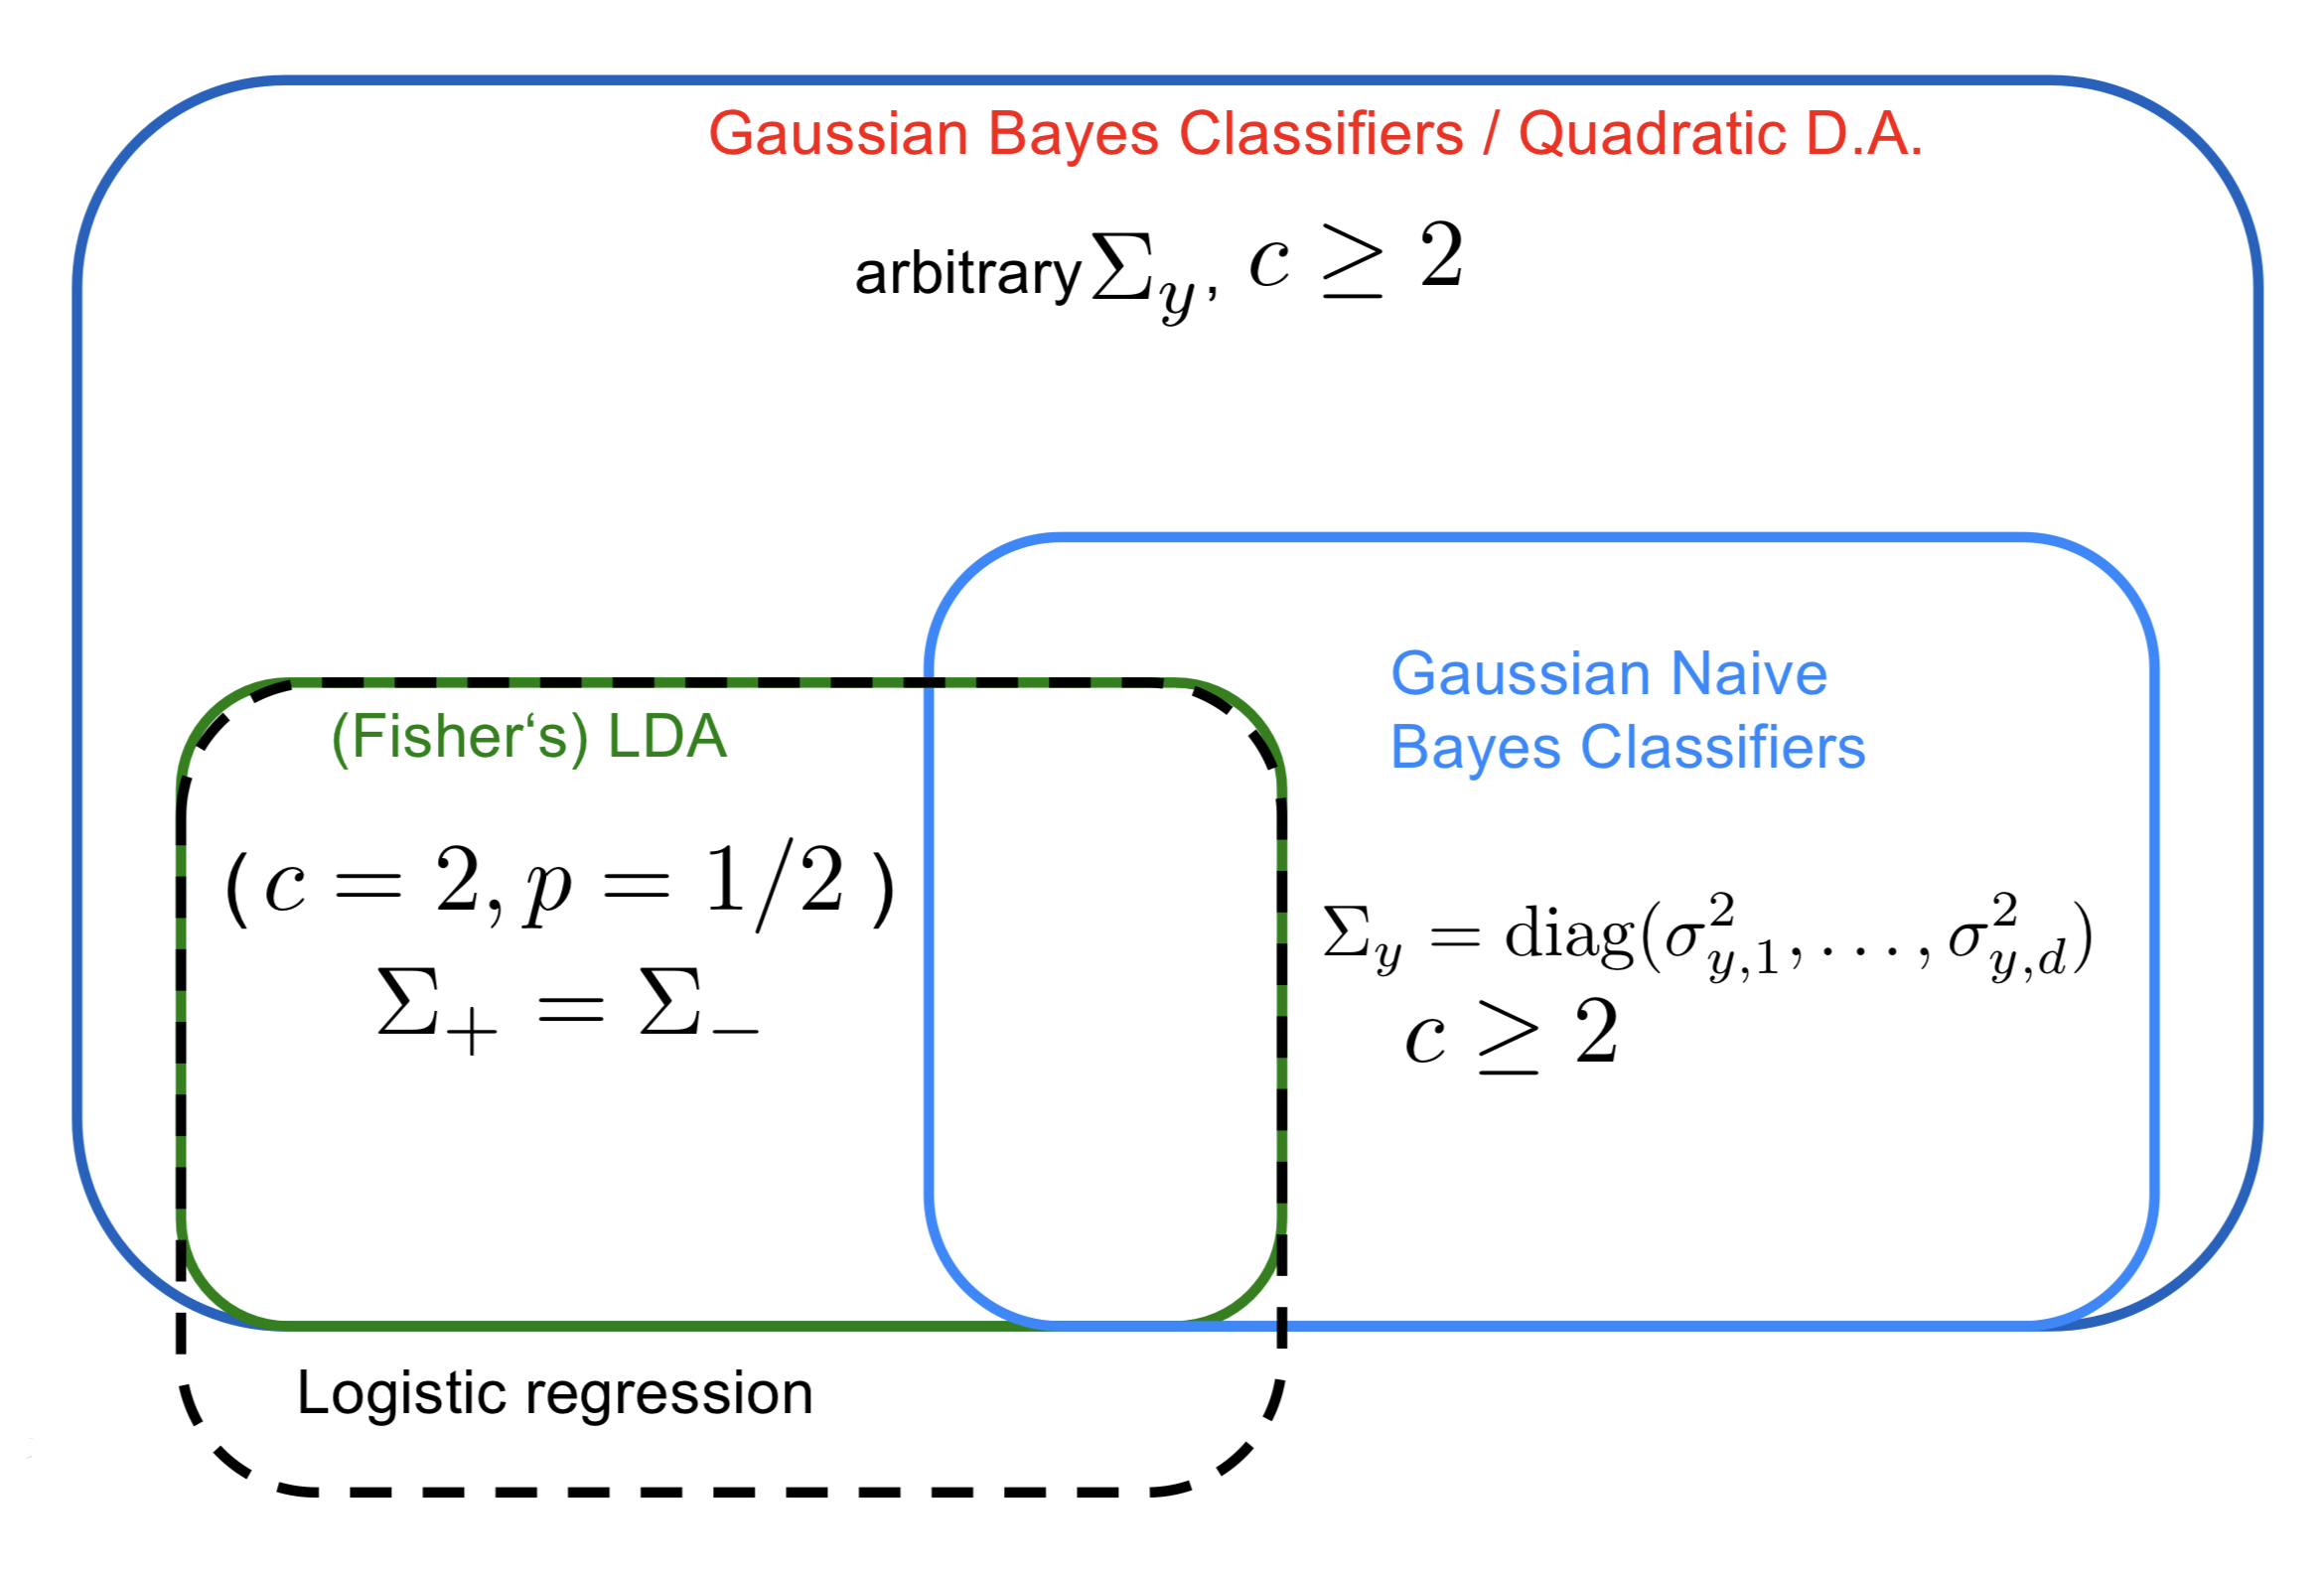
\includegraphics[width=\columnwidth]{qda-bigpicture.jpeg}
\end{center}

Gaussian Bayes classifiers can also be used for outlier detection by introducing a threshold $\tau$ such that all data points $x$ with $p(x) \leq \tau$ are outliers.

\subsection{Avoiding Overfitting}

From previous examples we know that MLE is prone to overfitting. We can avoid this by employing the techniques already seen:
\begin{itemize}
	\item Restricting Model Class: fewer parameters (e.g. GNB)
	\item Using Priors: restrict ("smaller") parameter values
\end{itemize}

Using a prior for the parameters leads us again to MAP estimation.

\subsection{Generative vs. Discriminative}

Discriminative models:
\begin{itemize}
	\item Model $p(y \; | \; x)$ and do not attempt to model $p(x,y)$
	\item Cannot detect outliers
	\item Are typically more robust, since accurately modeling $x$ may be difficult
\end{itemize}

Generative models:
\begin{itemize}
	\item Model joint distribution $p(x,y)$ and are therefore more ambitious
	\item Can be more powerful (e.g. dectect outliers, missing values) if model assumptions are met
	\item Are typically less robust against outliers
\end{itemize}

\section{Gaussian Mixture Model}

Gaussian mixture models make the assumption that data is generated from Gaussians. To be more precise a convex-combination of Gaussian distributions:
$$p(x \; | \; \theta) = p(x \; | \; \mu, \Sigma, w) = \sum_{j=1}^k w_j \cdot \mathcal{N}(x; \mu_j, \Sigma_j)$$

\begin{center}
	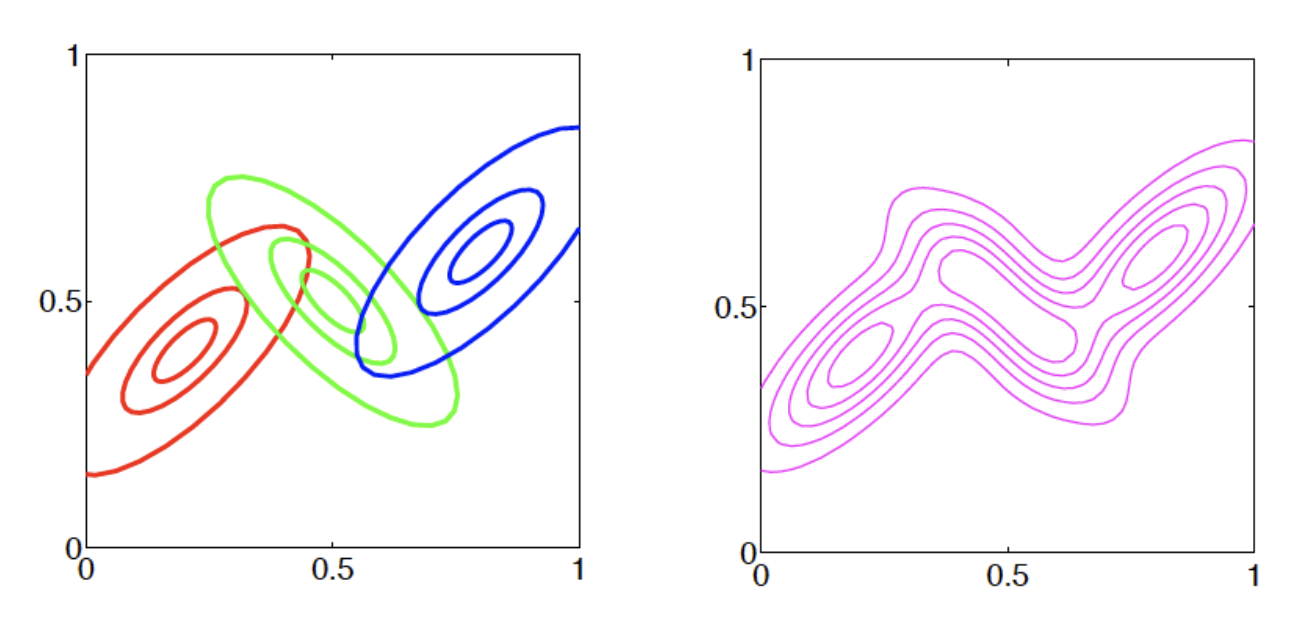
\includegraphics[width=\columnwidth]{gmm.png}
\end{center}

We do not know the labels $z$ for the data and can only see the level-set on the right, now we want to cluster this data. The problem we try to solve is to estimate the parameters for the Gaussian distributions (minimize log-likelihood).
$$(w_{i:k}^*, \mu_{i:k}^*, \Sigma_{1:k}^*) = \argmin \; - \sum_{i=1}^n \log \sum_{j=1}^k w_j \cdot \mathcal{N}(x_i \; | \; \mu_j, \Sigma_j)$$

This is a non-convex objective, but we can still try to apply SGD. But there is a better way to fit this model. The idea is that fitting a GMM is similar to training a GBC without labels. We want to apply an iterative approach where we first start with some guess for our parameters, predict the unknown labels and then impute the missing data. Now we can get a closed form update for our model which we then use to refine our parameters.

\subsection{Hard-EM Algorithm}

First we are gonna look at the simpler version of the EM (expectation maximization) algorithm:
\begin{itemize}
	\item Initialize the parameters $\theta^{(0)}$
	\item For $t = 1,2,...$ :
		\begin{itemize}
			\item \textbf{E-Step}: predict the most likely class for each data point:
				\begin{align*}
					z_i^{(t)} &= \argmax{z} \; p(z \; | \; x_i, \theta^{(t-1)}) \\
					&= \argmax{z} \; p(z \; | \; \theta^{(t-1)}) \cdot p(x_i \; | \; z, \theta^{(t-1)}))
				\end{align*}
			\item \textbf{M-Step}: compute MLE of $\theta^{(0)}$ as for GBC
		\end{itemize}
\end{itemize}

There are some problems with this approach, for one points are assigned a label even though the model is uncertain. Further it tries to extract too much information from a single point. In practice, this may work poorly if clusters are overlapping. Hard-EM with uniform weights and spherical covariances is equivalent to k-Means with Lloyd's heuristics.

\subsection{Soft-EM Algorithm}

Instead of predicting hard class assignments for each data point we want to predict class probabilities. 
\begin{itemize}
	\item Initialize the parameters $\theta^{(0)}$
	\item For $t = 1,2,...$ :
		\begin{itemize}
			\item \textbf{E-Step}: calculate the cluster membership weights for each point:
				\begin{align*}
					\gamma_j^{(t)}(x_i) &= p(z_i = j \; | \; x_i, \theta_j^{(t-1)}) \\
					&= \frac{w_j \cdot p(x_i ; \theta_j^{(t-1)})}{\sum_k w_k \cdot p(x_i ; \theta_k^{(t-1)})}
				\end{align*}
			\item \textbf{M-Step}: compute MLE with closed form solution:
				\begin{align*}
			 		w_j^{(t)} &= \frac{1}{n} \sum_{i=1}^n \gamma_j^{(t)}(x_i) \quad \; \mu_j^{(t)} = \frac{\sum_{i=1}^n x_i \cdot \gamma_j^{(t)}(x_i)}{\sum_{i=1}^n \gamma_j^{(t)}(x_i)} \\
			 		\Sigma_j^{(t)} &= \frac{\sum_{i=1}^n \gamma_j^{(t)}(x_i)(x_i - \mu_j^{(t)})(x_i - \mu_j^{(t)})^\top}{\sum_{i=1}^n \gamma_j^{(t)}(x_i)}
			 	\end{align*}
		\end{itemize}
\end{itemize}à

In general, Soft-EM will typically result in higher likelihood values, as it can better deal with "overlapping" clusters. When speaking of EM we usually refer to Soft-EM. \smallskip

The EM algorithm is sensitive to initialization. We usually initialize the weights as uniformly distributed, the means randomly or with k-Means++ and for variances we use spherical initialization or empirical covariance of the data. To select $k$, in contrast to k-Means, we can use cross-validation.

\subsection{Degeneracy of GMMs}

GMMs can overfit when only having limited data, we want to avoid that the Gaussians get too narrow and fit to a single data point. To avoid this we add $v^2 I$ to our variance. This makes sure that the variance does not collapse and is equivalent to placing a Wishart prior the covariance matrix, and computing the MAP. We choose $v$ by cross-validation.

\subsection{Gaussian-Mixture Bayes Classifiers}

We can also use GMMs for classification tasks, by assuming that the conditional distribution for each class can be modelled by a GMM.

$$p(x \; | \; y) = \sum_{j=1}^{k_y} w_j^{(y)} \mathcal{N}(x; \mu_j^{(y)}, \Sigma_j^{(y)})$$

We can then use this model for classification, giving us highly complex decision boundaries:

$$p(y \; | \; x) = \frac{1}{z} p(y)  \sum_{j=1}^{k_y} w_j^{(y)} \mathcal{N}(x; \mu_j^{(y)}, \Sigma_j^{(y)})$$

\begin{center}
	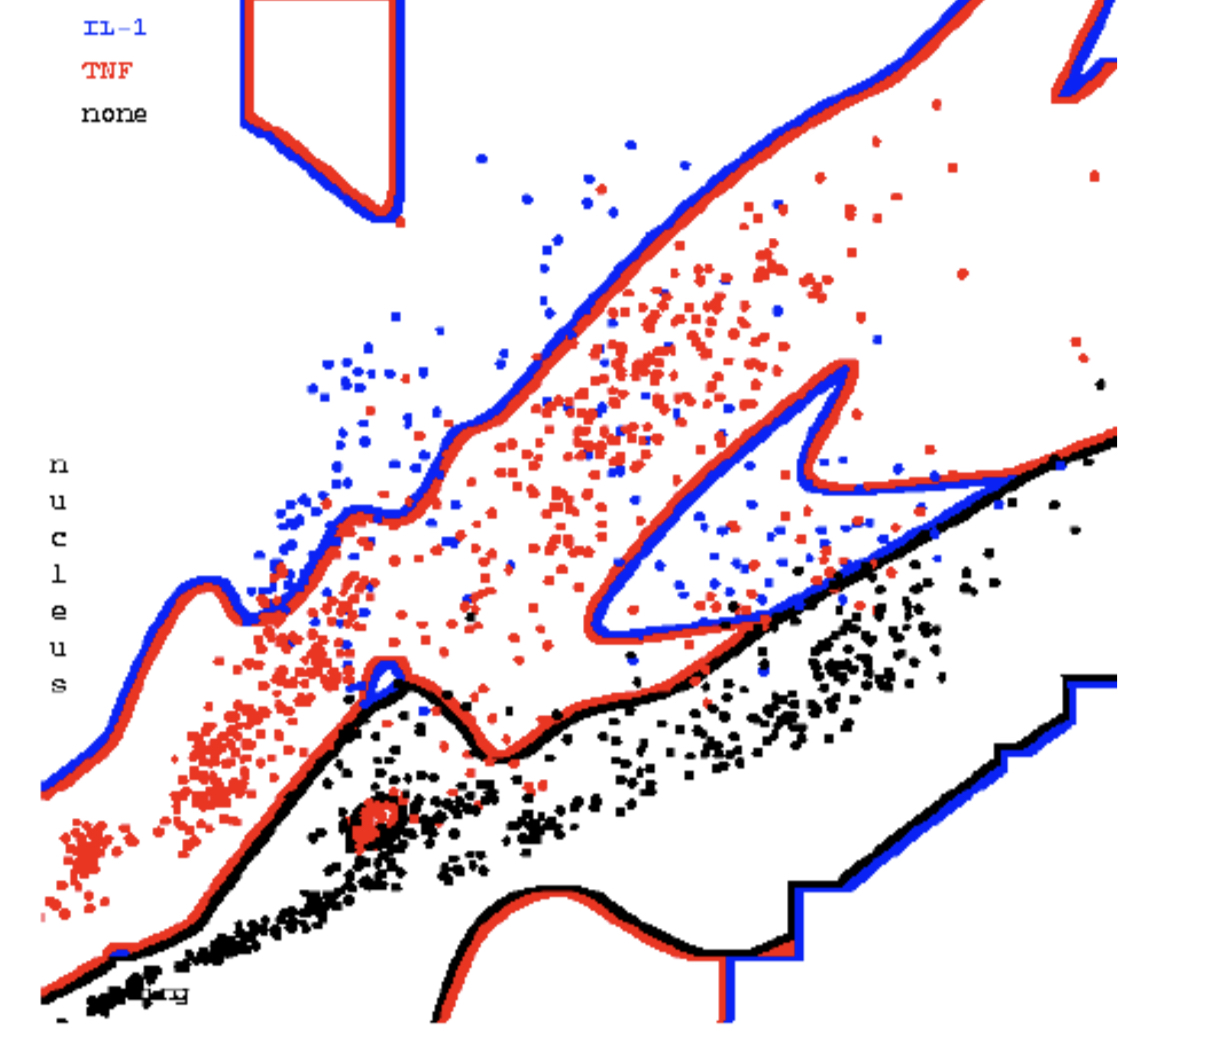
\includegraphics[width=0.7\columnwidth]{gmmb.jpeg}
\end{center}

\subsection{GMMs for Density Estimation}

So far, we used GMMs primarily for clustering and classification. Another natural use case for GMMs is density estimation, which in turn can be used for anomaly detection or data imputation.

\begin{center}
	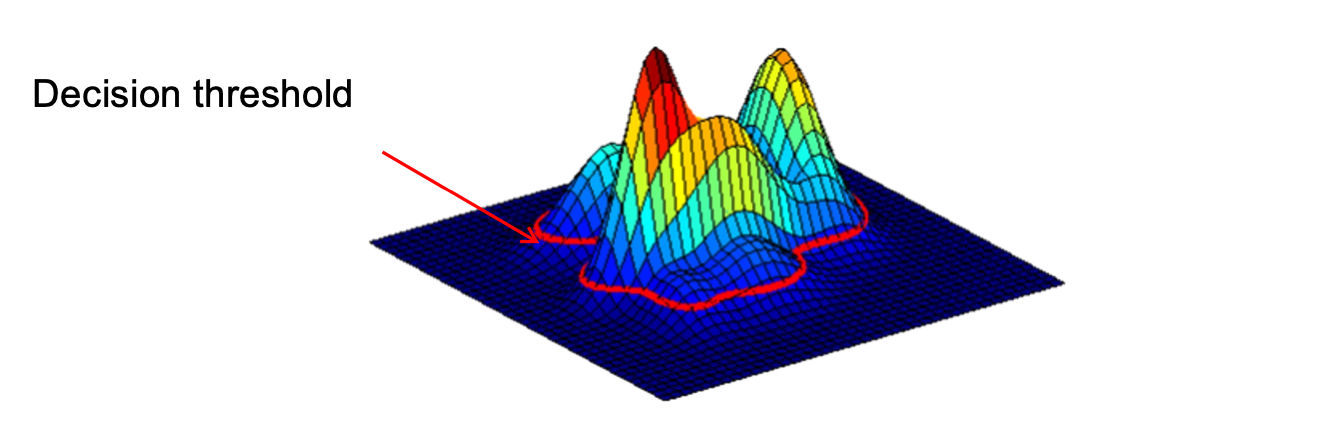
\includegraphics[width=\columnwidth]{anomaly-detection-gmm.png}
\end{center}

To determine outliers, we simply compare the estimated density of a data point against a threshold value $\tau$. This allows us to control the FP rate. As we vary the threshold we trade FPs and FNs. We can use ROC curves as evaluation criterion and optimize using cross-validation to find the optimal value for $\tau$.

\subsection{General EM Algorithm}

The framework of soft EM can also be used for more general distributions than gaussians. We formulate the two steps:
\begin{itemize}
	\item \textbf{E-Step}: Take the \textbf{expected} value over latent variables to generate a likelihood function $Q(\theta ; \theta^{(t-1)})$:
		\begin{align*}
			Q(\theta ; \theta^{(t-1)}) &= \E_{Z}[ \log  p(X, Z \; | \; \theta) \; | \; X, \theta^{(t-1)}] \\
			&= \sum_{i=1}^n \sum_{z_i=1}^k \gamma_{z_i}(x_i) \log p(x_i, z_i \; | \; \theta)
		\end{align*}
		with $\gamma_z(x) = p(z \; | \; x, \theta^{(t-1)})$
	\item \textbf{M-Step}: Compute MLE / \textbf{Maximize}:
		$$\theta^{(t)} = \argmax{\theta} \; Q(\theta; \theta^{(t-1)})$$
\end{itemize}

It is important to note that we have guaranteed mono- tonic convergence, where each EM-iteration monotonically increases the data likelihood.

\section{Generative Adversarial Networks}

Until now the models we explored failed to capture complex, high-dimensional data types (e.g. images and audio). The key idea is to use a neural network to learn a function that takes a "simple" distribution (e.g. Gaussian) and returns a non linear distribution. This leads us to the problem that it becomes to compute the likelihood of the data needed for the loss. Therefore we need an alternative objective for training.

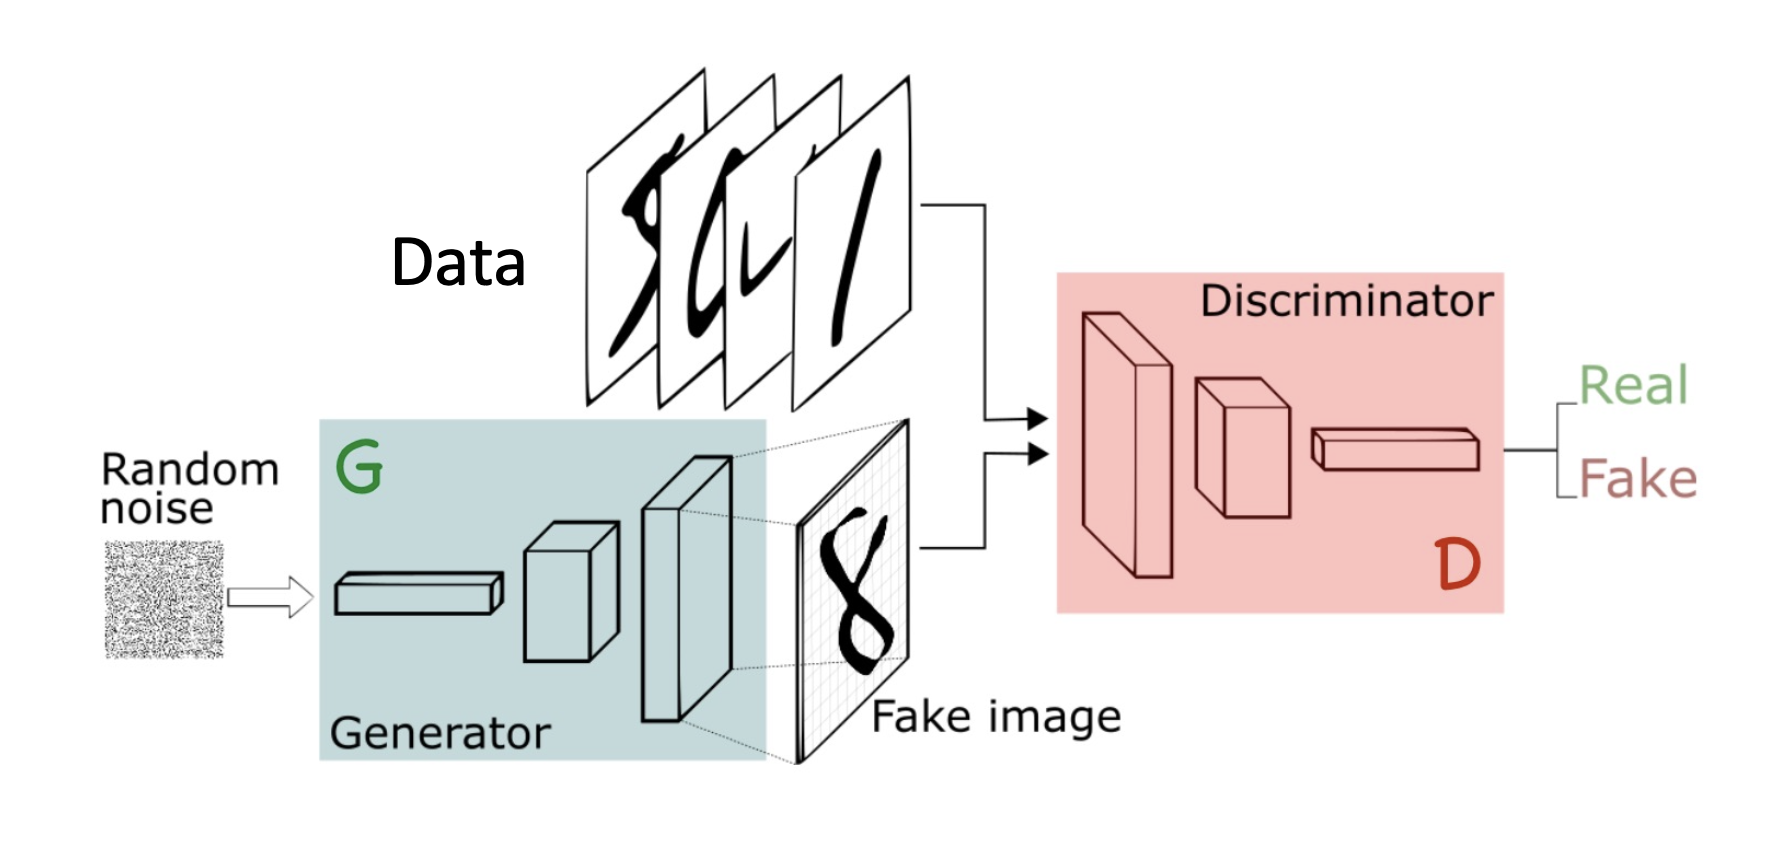
\includegraphics[width=\columnwidth]{gan.png}

We simultaneously train two neural networks, a generator $G$ trying to produce realistic examples and a discriminator $D$ trying to detect "fake" examples. This whole process can be viewed as a game, where the generator and discriminator try to compete against each other. This leads to the following objective:

\begin{align*}
	\min_{w_G} \max_{w_D} \; & \E_{x \sim p_{\text{data}}} [\log D(x, w_D)] \\
 	+ &\E_{z \sim p_z} [\log (1 - D(G(z, w_G), w_D))]
 \end{align*}
 
 Training a GAN requires to find the saddle point rather than a (local) minima. For a fixed generator $G$, the optimal discriminator is such that:
 $$D_G(x) = \frac{p_{\text{data}}(x)}{p_{\text{data}}(x) + p_G(x)}$$
 
 In general it is important that the discriminator is not too powerful, as this could lead to memorization on finite data. Other issues that can occur are oscillations/divergence or mode collapse. \medskip
 
 Evaluation GANs is still an open research question. One possible performance metric is the so called duality gap:
 $$DG(w_G, w_D) = \max_{w_D'} M(w_G, w_D') - \min_{w_G'} M(w_G', w_D)$$
 
 Where $M(w_G, w_D)$ is the objective used in training.
 

\end{multicols*}
\end{document}

% ____ FOOTER ______________________________________________________
% Content and Template: 
% original by Danny Camenisch (dcamenisch@inf.ethz.ch), 2022
% based on different summaries from many helpful people